
% Copyright 2007, 2008, 2009 Elsevier Ltd 
% 
% This file is part of the 'Elsarticle Bundle'.
% --------------------------------------------- 
%
% It may be distributed under the conditions of the LaTeX Project Public
% License, either version 1.2 of this license or (at your option) any
% later version.  The latest version of this license is in
%    http://www.latex-project.org/lppl.txt
% and version 1.2 or later is part of all distributions of LaTeX
% version 1999/12/01 or later c.
%
% The list of all files belonging to the 'Elsarticle Bundle' is
% given in the file `manifest.txt'.
%
 
% Template article for Elsevier's document class `elsarticle'
% with harvard style bibliographic references
% SP 2008/03/01
%
%
%
% $Id: elsarticle-template-harv.tex 4 2009-10-24 08:22:58Z rishi $
%
%
%\documentclass[preprint,authoryear,12pt]{elsarticle}
\documentclass[preprint,12pt]{elsarticle}

% Use the option review to obtain double line spacing
%\documentclass[authoryear,preprint,review,12pt]{elsarticle}

% Use the options 1p,twocolumn; 3p; 3p,twocolumn; 5p; or 5p,twocolumn
% for a journal layout:
%\documentclass[final,authoryear,1p,times]{elsarticle}
%\documentclass[final,authoryear,1p,times,twocolumn]{elsarticle}
%\documentclass[final,authoryear,3p,times]{elsarticle}
%\documentclass[final,authoryear,3p,times,twocolumn]{elsarticle}
%\documentclass[final,authoryear,5p,times]{elsarticle}
%\documentclass[final,authoryear,5p,times,twocolumn]{elsarticle}

%% if you use PostScript figures in your article
%% use the gra

%%graphis package for simple commands
%% \usepackage{graphics}
%\usepackage{cases}
%% or use the graphicx package for more complicated commands
\usepackage{graphicx}
%% or use the epsfig package if you prefer to use the old commands
\usepackage{epsfig}
%\usepackage{subfig}
\usepackage{comment}

\usepackage{epstopdf}
\usepackage{pdflscape}
\usepackage{bm}
\usepackage{hyperref,url}
\hypersetup{colorlinks=true, urlcolor=blue, linkcolor=blue, citecolor=red}

%% The amssymb package provides various useful mathematical symbols

\usepackage{amssymb,amsmath,array}
%The amsthm package provides extended theorem environments

\usepackage{amsthm}
\usepackage{graphicx}
%\usepackage{subfigure}
  
%% The lineno packages adds line numbers. Start line numbering with
%% \begin{linenumbers}, end it with \end{linenumbers}. Or switch it on
%% for the whole article with \linenumbers after \end{frontmatter}.
%% \usepackage{lineno}

\usepackage{lscape}

%% natbib.sty is loaded by default. However, natbib options can be
%% provided with \biboptions{...} command. Following options are
%% valid:

%%   round  -  round parentheses are used (default)
%%   square -  square brackets are used   [option]
%%   curly  -  curly braces are used      {option}
%%   angle  -  angle brackets are used    <option>
%%   semicolon  -  multiple citations separated by semi-colon (default)
%%   colon  - same as semicolon, an earlier confusion
%%   comma  -  separated by comma
%%   authoryear - selects author-year citations (default)
%%   numbers-  selects numerical citations
%%   super  -  numerical citations as superscripts
%%   sort   -  sorts multiple citations according to order in ref. list
%%   sort&compress   -  like sort, but also compresses numerical citations
%%   compress - compresses without sorting
%%   longnamesfirst  -  makes first citation full author list
%%
%% \biboptions{longnamesfirst,comma}

% \biboptions{}

\newcommand{\JGnote}[1]{\fbox{\parbox{\textwidth}{ \color{red} JG Note $\Rightarrow$ #1}}}
\newcommand{\BLnote}[1]{\fbox{\parbox{\textwidth}{ \color{green} BL Note $\Rightarrow$ #1}}}
\newcommand{\red}{\textcolor{red}}
\newcommand{\blue}{\textcolor{blue}}
\newcommand{\green}{\textcolor{green}}
\newcommand{\yellow}{\textcolor{yellow}}
\newcommand{\frc}{\displaystyle\frac}
\newcommand{\PN}[2][error]{P$_{#1}$DG-P$_{#2}$}
\newcommand{\PNDG}[2][error]{P$_{#1}$DG-P$_{#2}$DG}
\newcommand{\eg}{{\it e.g., }} 
\newcommand{\ie}{{\it i.e., }}
\newcommand{\st}{{\it s.t., }}

\journal{Applied Mathematical Modelling}

\begin{document}

\begin{frontmatter}

%% Title, authors and addresses

%% use the tnoteref command within \title for footnotes;
%% use the tnotetext command for the associated footnote;
%% use the fnref command within \author or \address for footnotes;
%% use the fntext command for the associated footnote;
%% use the corref command within \author for corresponding author footnotes;
%% use the cortext command for the associated footnote;
%% use the ead command for the email address,
%% and the form \ead[url] for the home page:
%%
%% \title{Title\tnoteref{label1}}
%% \tnotetext[label1]{}
%% \author{Name\corref{cor1}\fnref{label2}}
%% \ead{email address}
%% \ead[url]{home page}
%% \fntext[label2]{}
%% \cortext[cor1]{}
%% \address{Address\fnref{label3}} 
%% \fntext[label3]{}

\title{A Reduced Order Model for Permeability Fields Using Singular Value Decomposition (SVD)}
\author[UoA]{B. Lashore}\ead{lashorebabatunde@yahoo.com} \author[UoA]{K. Christou} \author[UoA]{J.L.M.A. Gomes\corref{cor1}}\ead{jefferson.gomes@abdn.ac.uk}
%\author[UoA]{B. Lashore\corref{cor1}}\ead{lashorebabatunde@yahoo.com} \author[UoA]{K. Christou} \author[UoA]{J.L.M.A. Gomes} 
\cortext[cor1]{Corresponding author.}
\address[UoA]{Mechanics of Fluids, Soils \& Structures Research Group \\ School of Engineering, University of Aberdeen, UK}


\begin{abstract}

Representation of heterogeneous properties (\ie permeability in this case) within a large system, is a challenge that cuts across many industries that deal with flow in porous media. This is because it is impossible to obtain the value of permeability at every point in realistic domain. And, even if this was possible, it would be extremely challenging to get the computing resources to make use of all this data. This challenge gave birth to upscaling, a model order reduction method.

In this paper, a SVD-based method was developed to reduce the order of porous media permeability field (\ie upscale). This method was compared to traditional industry-standard upscaling techniques (\eg arithmetic and harmonic averaging) and to a stochastic-based (probability density function, PDF) method of upscaling, to highlight its benefits performance. It was shown that the SVD upscaling technique retained the heterogenous nature of the BaseCase (\ie high-resolution configuration). Additionally, the SVD upscaling technique did not require {\it a priori} understanding of similar permeability blocks within the existing domain.

\end{abstract}



\begin{keyword} %% keywords here, in the form: keyword \sep keyword
Singular Value Decomposition (SVD)\sep Upscaling\sep Model Order Reduction (MOR) \sep  Principal Component Spaces \sep Permeability field \sep Heterogeneity
\end{keyword}
 
\end{frontmatter}

%%%%%%%%%%%%%%%%%%%%%%%%%%%%%%%%%%%%%%%%%%%%%%%%%%%%%%%%%%%%%%%%%%%%%%%%%%%%%%%%%%%%%%%%%%%%%%%%%%%%%%%%%%%%%%%%%%%%%%%%%%%%%%%%%%%%%%%%%%%%%%%%%%%%%%%%%%%%%%%%%%%%%%%%%%%%%%%%%%%%%%%%%%%%%%%%%%% 
\section{Introduction}\label{section:intro}
Naturally occuring rock formations are inherently heterogeneous, which means that rock properties such as permeability, pore spaces (\ie porosity) and pore throat vary spatially at different length scales. Heterogeneity of rock formations is relevant in calculations of transport and storage of fluids in porous media (\ie multiphase flow in subsurface rocks). Therefore, the representation of such heterogeneous properties is of great importance to oil and gas (\ie reservoir management), carbon capture and storage (CCS, \ie CO$_2$ transportation and storage in subsurface rocks) and waste management (\ie remediation of contaminated soil).

In essence, rock heterogeneity makes it impossible to obtain reliable and accurate spatial information about geological properties throughout the domain (\ie uncertainty problem). Additionally, due to limitations in computing resources, it is neither efficient nor possible to use exact values of geological properties at all spatial coordinates of the domain to perform fine-grid simulations (\ie scaling problem) \cite{chen_2006,miller_1998,Renard_1997}. This is particularly true for large geological domains which span several kilometres. It is possible to overcome these challenges by a family of techniques called {\it upscaling}. Upscaling techniques solve both uncertainty and scaling problems by replacing discrete geological and fluid properties of detailed high resolution domains with coarse descriptions (low resolution) of these properties \cite{Vereecken_2007}.

Upscaling techniques which best preserve statistical properties and flow dynamics behaviour of the high resolution domain give the best representation of heterogeneous properties. There are several upscaling techniques which fall under different categories \cite{Hasting_2001, Renard_1997, Szymkiewicz_2013}. Traditional upscaling techniques are deterministic in nature, however over the last decade, techniques classed as stochastic have received great attention from academic and industrial porous media communities worldwide \cite{Guilleminot_2012, Ravalec-Dupin_2010, Verwoerd_2009}. One of the reasons for this is because stochastic upscaling techniques are robust enough to handle multiphase flow in porous media and they are able to address scaling and uncertainity problems.

\medskip
{\it Upscaling} is a term commonly used in the oil and gas sector and is often referred, throughout the applied mathematics and engineering communities, as a form of model order reduction (or reduced order models, MOR/ROM). Depending on the context in which MOR is used, it can simply be referred as dimensionality reduction. The definition of MOR also depends on the context it is being used, but it suffices to state that MOR captures the essential features of a system, structure or parameter \cite{Schilders2008}. This implies that an original system exists with more detailed information. Figure~\ref{fig:IllustrationMOR} presents an interpretation of MOR concept in which a graphical representation of a rabbit is reconstructed with a reduced number of facets (rhs of this illustration).  

\citet{Schilders2008} provided a historical perspective on the development of Model Order Reduction, from the work of Fourier in 1807 which approximated a function with a few trigonometric terms, to the work of \citet{Odabasioglu_1998} in 1998 which introduced Passive Reduced-order Interconnect Macromodeling Algorithm (PRIMA). Truncated Balanced Realization  is another MOR method developed by \citeauthor{Moore_1981}~\cite{Moore_1981}, which introduced the principal component analysis \cite{Hotelling_1933} and \citeauthor{Golub1970}'s \cite{Golub1970} algorithm for solving singular value decomposition (SVD). Hankel-norm reduction \cite{Glover_1984} and Proper Orthogonal Decomposition \cite{Sirovich_1987} are also MOR methods discussed in the referenced articles published in 1984 and 1987 respectively. The asymptotic waveform evaluation (AWE) \cite{Pillage_1990} was the first MOR method based on Krylov subspace technique, this method was followed by Pade-via-Lanczos method \cite{Feldmann_1995} and the PRIMA. In this work, upscaling is performed by SVD in principal component spaces.

\bigskip
This work focuses on reducing the order of permeability distribution in porous media flow simulations. Section~\ref{section:mathematical_model} introduces the mathematical model used to describe the relevant physics for multi-fluid flow through porous media and highlights the relevance of the permeability field. The mathematical model is discretised by a novel high-order accurate control volume finite element method (CVFEM) \cite{Gomes_2017} which couples both the fine resolution and upscaled representation of the permeability field. Pre-processing statistical properties and post-simulation multiphase flow behaviour are investigated to assess the various upscaling techniques used.

Four upscaling techniques are investigated in this work, arithmetic and harmonic means are used to obtain the first two upscaled representation and these two are classed as deterministic techniques. The third is a randomly generated permeability field with Gaussian distribution, prescribed by a probability density function (PDF) which was obtained from a domain discretised with high-resolution mesh with known permeability distribution (\ie base case). The fourth upscaling technique is the crux of this research, it introduces singular value decomposition (SVD) as a method of upscaling using the concept of principal component space to reduce the order of the permeability distribution.

In Section~\ref{section:svd}, fundamental mathematics of SVD and associated properties are presented. Then, the concept of spaces is explained to give the reader the understanding necessary to appreciate the transformations and projections involved in this work. Finally, Section~\ref{section:svd} describes model order space reduction for the permeability field within the principal component space. Section~\ref{section:model_simulation} starts by describing the high resolution (\ie base case) on which the four upscaling techniques are applied to. A brief summary of the pre-processing step for each of the models is also presented. Section~\ref{section:results_discussion} provides the results and further discussion on the results of the simulations, it also gives further interpretation to the result obtained from the SVD upscaling technique. Finally, Conclusions are drawn in Section~\ref{section:conclusion}.

\section{Mathematical Model}\label{section:mathematical_model}

\citet{Gomes_2017} provides details on the governing equations and numerical formulation which forms the mathematical model for the multi-flow flow in this work. Albeit, it suffices to introduce only the representation of Darcy's law for immiscible multi-phase flow for the following discussion. This is written in the form:
\begin{equation}\label{e:darcy_eqn}
  \mathbf{q}_{\alpha} =
  -\frac{\mathcal{K}_{{r}_\alpha}\mathbf{K}}{\mu_{\alpha}}\left(
  \nabla p_{\alpha} - {\mathbf{s}_{u}}_{\alpha} \right),
\end{equation}
where $\alpha$ designates a phase and $\mathbf{q}_{\alpha}$ is the $\alpha$-th phase Darcy velocity. $\mu_{\alpha}$, $p_{\alpha}$, $\rho_{\alpha}$, and $\mathbf{s}_{{u}_\alpha}$ are the phase dynamic viscosity, pressure, density and source term, which may include gravity and/or capillarity, respectively. $\mathcal{K}_{{r}_\alpha}\left(S_{\alpha}\right)$ is the phase relative permeability, which is a function of the phase saturation $S_{\alpha}\left(\mathbf{r},t\right)$, which in turn is a function of the vector position $\mathbf{r}$, and time, $t$. Finally, $\mathbf{K}\left(\mathbf{r}\right)$, the focus of this work, is the absolute permeability tensor of the porous medium and it is a function of the vector position $\mathbf{r}$.

In this work, $\mathbf{K}$ is prescribed in the system of governing equations used to model multi-phase flow in porous media, this means it is an input/independent variable. Since $\mathbf{K}$ varies with position, it is impossible to determine at every point and even if it is available at every point it would require immense computer resources to utilize all the available information in a simulation. This is the reason upscaling is required for the permeability field. Upscaling can be performed from the continuum scale, across the micro scale ($mm$), local scale and meso scale ($m$) to the field scale ($Km$)\cite{ECMI_2004}. The upscaling discussed here is from the micro scale also known as the Darcy scale.

\section{Brief Overview of Upscaling}\label{section:overview_upscaling}

Section~\ref{section:intro} briefly introduced the rational behind upscaling. Upscaling methods replace discrete geological and fluid properties of detailed high resolution domains with coarse descriptions (low resolution) of these properties \cite{Vereecken_2007}. This subject of upscaling heterogenous properties has interested industries (\ie oil and gas, CCS and waste management) as well as the academic community for over $7$ decades.

Those interested in large-scale reservoirs or ground water generally take a two-stage geostatistical approach to be subject. In the first stage, information from seismic data, well data and analogous outcrops is used to model the large scale heterogeneities associated with facies. And in the second stage, statistical models such as continuous multi-variate Gaussian field is used to model the rock properties of the facies \cite{Ewing_1997}. In addition to seismic and well data used in the previous stage, core data can be used as a sources of information for the statistical properties used to determine the random field in this stage.

A lot of work has been carried out on the upscaling of permeability fields \cite{Christie_2001SPE10Model, Ewing_1997, Hasting_2001, King1996, Indelman_1993, Vereecken_2007, Wen_1996, Yeo2001}. \citet{Cardwell_1945} investigated arithmetic and weighted averages as upscaling techniques for calculating a single equivalent permeability for an oil reservoir with varying permeabilities. The general conclusion reached from this study was that the equivalent permeability lies between the harmonic and the arithmetic average.  

\citet{Yeo2001} discussed the accuracy of renormalization method for upscaling 2D hydraulic conductivity fields for two cases. Both cases employed the $4$-quadrant model (see Section~\ref{subsection:model} for details) set-up. The first case had low permeablitity in all the blocks except the bottom right block which had high permeability, while the second case employed the checkboard style described in Section~\ref{subsection:model}. Different conductivity ratios were also investigated for the two cases. The conclusion drawn was that renormalization worked fairly well for the first case, but very poorly for the second case.

\citet{Renard_1997} provided a comprehensive review of the various techniques for upscaling. He found out that the techniques classed broadly under deterministic, stochastic and heuristic complemented each other rather than antagonising each other. \citet{Renard_1997} then recommended that it is better to select a technique which provides block permeabilities instead of one which provides uniform effective permeability.

\citet{Christie_2001SPE10Model} provided $2$ sets of problems to compare the upscaling and upgridding techniques of different simulators. The paper does not describe in any detail the upscaling techniques used by the different simulators, but it provides a complete dataset for running simulations.


\section{Singular Value Decomposition, SVD, and its application for reducing the order of a permeability field}\label{section:svd}
\subsection{A Brief Introduction to SVD}\label{subsection:svd_brief}
Given a matrix $\mathbf{A}\in\mathcal{R}^{m\times n}$, the singular value decomposition (SVD) is a method for factorizing $\mathbf{A}$, such that,
\begin{equation}
  \mathbf{A} = \mathbf{U}\mathbf{\Sigma}\mathbf{V}^{\intercal}.
\end{equation}
where $\mathbf{U}=\left[\underline{u}_{1},\underline{u}_{2},\cdots,\underline{u}_{m}\right]\in\mathcal{R}^{m\times n}$ and $\mathbf{V}=\left[\underline{v}_{1},\underline{v}_{2},\cdots,\underline{v}_{n}\right]\in\mathcal{R}^{m\times n}$ are orthogonal but not necessarily the same. $\Sigma$ is a diagonal matrix, \ie $\Sigma=\text{diag}\left(\sigma_{1},\sigma_{2},\cdots,\sigma_{r}\right)\in\mathcal{R}^{m\times n}$ and $r=\min\left\{m,n\right\}$ is the rank of $\mathbf{A}$, with $\sigma_{1}\ge\sigma_{2}\ge\cdots\sigma_{r}\ge 0$. The diagonal entries of $\Sigma$ $\left(\ie \sigma_{i}, i=1,r\right)$ are called singular values of $\mathbf{A}$. If $\mathbf{A}$ is a square matrix then $\mathbf{U}$, $\Sigma$ and $\mathbf{V}$ are also square matrices. Also, as $\mathbf{U}$ and $\mathbf{V}$ are orthogonals and unitary, 
\begin{equation}
  \mathbf{U}^{\intercal}\mathbf{U} = \mathbf{V}^{\intercal}\mathbf{V} = \mathbf{I},
\end{equation}
where $\mathbf{I}$ is an identity matrix. However, if $\mathbf{A}$ is an $m\times n$ matrix, $\mathbf{U}$ and $\mathbf{V}$ still remain as square matrices, albeit with different matricial sizes. $\mathbf{U}$ is an $m\times m$ while $\mathbf{V}$ is an $n\times n$. Another relevant property of $\mathbf{U}$ and $\mathbf{V}$ since they are square (irrespective of whether $\mathbf{A}$ is square or rectangular) is that
\begin{equation}
  \mathbf{U}^{-1} = \mathbf{U}^{\intercal} \;\;\;\text{ and }\;\;\; \mathbf{V}^{-1} = \mathbf{V}^{\intercal},
\end{equation}
and if $\mathbf{A}$ is an $m \times n$ matrix thus $\Sigma$ is a diagonal $m \times n$ matrix. For a rectangular matrix, the singular values fill the first $r$ places on the main diagonal of $\Sigma$. The SVD benefits from the orthogonality of the columns in $\mathbf{U}$ and $\mathbf{V}$. The columns of $\mathbf{U}$ are known as the left singular vectors while the columns in $\mathbf{V}$ are known as the right singular vectors. A simple consideration of the benefit of the orthogonal factors, $\mathbf{U}$ and $\mathbf{V}$, is the ease with which they allow the inverse of the square matrix $\mathbf{A}$ to be calculated. This in turn makes it easy to solve the linear Equ.~\ref{e:Ax=b} for $x$. Equ.~\ref{e:SVD_factorization} show the SVD factorization already discussed, and with benefit of the orthogonal property also already discussed, the solution for $x$ is simply presented as in Equ.~\ref{e:x_solution}.
\begin{equation}\label{e:Ax=b}
 \mathbf{A}x = b
\end{equation}
\begin{equation}\label{e:SVD_factorization}
 \mathbf{U} \Sigma \mathbf{V}^{\intercal} x = b
\end{equation}
\begin{equation}\label{e:x_solution}
 x = \mathbf{V} \Sigma^{-1} \mathbf{U}^{\intercal} b
\end{equation}


\subsection{Principal Component Spaces and Model Order Reduction for the permeability field}\label{subsection:pcspaces}
  
\subsubsection{Understanding the permeability space}\label{subsubsection:visualization_permspace}
In 3D geometry, permeability is a tensor quantity, but for the purpose of the following explanation (and the remaining part of this paper), a 2D geometry is assumed where permeability is a scalar quantity. Furthermore, the simulator prescribes the permeability field by assigning permeability values in the centre of the elements/cells which discretizing the 2D simulation domain. The permeability value assigned in the centre of the element/cell represents the permeability value for that element/cell. For simplicity, in the remaining part of this section, it will be assumed that the $2D$ geometry is discritized by a square grid with the value for each square element assigned in the centre of the element. This explanation allow one to easily visualize this permeability space because it is defined by the cartesian coordinates  system which most people are already familiar with. The model order reduction for the permeability field discussed here is concerned with reducing the volume of permeability data within the permeability space. Consider for instance a small square which is discretized to contain four squares such that $4$ data values are defined in the middle of the four squares. The permeability space of $4$ can be reduced to a smaller value of $1$ through an averaging process such as arithmetic, harmonic or geometric mean. This type of reduction is the focus of this paper, albeit the main focus of this paper is achieving this reduction through singular value decomposition in the principal component spaces. 

\subsubsection{Understanding the principal component spaces}\label{subsubsection:visualization_pcspaces}
Essentially, the existing permeability space is transformed through SVD to principal component spaces where usually, traditional principal component analysis is performed before interpolation is used to implement further data reduction in the principal component spaces. This reduced data in the principal component space is then transformed back into the permeability space to obtain a reduced permeability space.

The principal component space is more challenging to visualize because it usually consists of more than $3$ dimensions. $3-D$ ({\it i.e.}, $x, y$ and $z$ in the cartesian plane) being the natural dimension which humans exist, is easy to visualize. Many individuals are also able to understand the concept of 4D with time as the fourth dimension, albeit only few scientists and engineers are able to visualize and work in the abstract dimension where the number of dimensions exceed four. An aid for visualizing the PC space is to write out the $\mathbf{U}$, $\mathbf{\Sigma}$ and $\mathbf{V^{\intercal}}$ matrices (or imagine the matrices written out) and consider the singular vectors ({\it i.e.},columns in $\mathbf{U}$ and rows in $\mathbf{U}$) as separate principal component spaces.

\subsubsection{Model Order Reduction/Principal Component Space Reduction}\label{subsubsection:svdcase_preprocess_algorithm}
 For the SVD model order reduction of the permeability field, all the work is done in the principal component spaces. This can be completed in two steps. The first step is optional and it is the well known principal component analysis (PCA) \cite{Hotelling_1933}. Here, the singular values are examined and based on a pre-defined criteria, $z$ singular values are selected, starting from $\sigma_{1}$ and in a decreasing order, where $z \leq r$. In the case with $z = r$, it can be assumed that step 1 has been ignored. However, when $z < r$, the first $z$ columns of $\mathbf{U}$ and the first $z$ rows of $\mathbf{V^{\intercal}}$ are extracted from $\mathbf{U}$ and $\mathbf{V^{\intercal}}$ to form new matrices $\mathbf{U_{new}}$ and $\mathbf{V^{\intercal}_{new}}$ respectively. The selected $z$ singular values also form a new diagonal matrix, $\mathbf{\Sigma_{new}}$ .

The second step involves interpolation within each singular vector (column in $\mathbf{U}$ and row in $\mathbf{V^{\intercal}}$), to reduce the number of data in each column of  $\mathbf{U}$ and in $\mathbf{V^{\intercal}}$. From this step,  $\mathbf{U_{new2}}$ and $\mathbf{V^{\intercal}_{new2}}$ are obtained. The reduced permeability field is calculated by multiplying  $\mathbf{U_{new2}}$, $\mathbf{\Sigma_{new}}$ and $\mathbf{V^{\intercal}_{new2}}$. 


\section{Model Description and Simulation Setup}\label{section:model_simulation}

\subsection{Model Description}\label{subsection:model}
The BaseCase  ({\it i.e.} fine resolution) model for the permeabiliy field builds on the $2 \times 2$ block, $4$ quadrant model used initially by \citet{Cardwell_1945} and later by \citet{Yeo2001} and \citet{dawe_2008}. These authors designed the permeability field for the quadrants in a checkerboard style which means that diagonally opposite blocks retained the same permeability values with one set of diagonally opposite blocks having a higher permeability value compared to the other set. Hence, one set of diagonally opposite blocks are referred to as high permeability blocks while the other set is referred to as low permeability blocks. The BaseCase permeability model used in this manuscript retains the checkerboard desgined used by the recently named authors. Albeit, the permeability data for each block in the set of diagonally opposite blocks have similar value ({\it i.e.} not exactly the same as in the papers referred to), although one set can still be referred to as a set of high permeability blocks while the other set is referred to as a set of low permeability blocks. Furthermore, within each block, the permeability field varies within a pre-defined range and consists of $1600$ permeability values. More details on the design of the permeability field for the BaseCase is available in section~\ref{subsubsection:basecase_preprocess_algorithm}. And Fig.~\ref{fig:PermFields}a and~\ref{fig:PermFields}b give a pictorial representation of the permeability field for the base case with the mesh discretization visible and invisible respectively. Using the labelling scheme used by \citet{dawe_2008}, the quadrant model block $K1,~K2,~K3$ and $K4$ are top left, bottom left, top right and bottom right respectively.

As already mentioned, four upscaled permeability field models were obtained from the high-resolution ({\it i.e.} the BaseCase) permeability field. When compared to the BaseCase model, all the upscaled models were upgridded to reduce the resolution of the permeability field (Fig.~\ref{fig:HiRes_LowRes_Mesh}). The first two upscaled models are referred to as the ArithMean and the HarmMean Cases, and this is because they are based on the arithmetic and the harmonic averaging methods, respectively. In both the ArithMean and HarmMean Cases, averages are calculated for each block using the $1600$ data points from the blocks of the BaseCase to obtain a permeability value for each block in the upscaled models. This effectively homogenizes the permeability field in each block. The upscaled permeability field for the third and fourth cases are referred to as PDFCase and SVDCase, respectively. And, as can be deduced from the names, these cases are based on probability density function (PDF) and singular value decomposition (SVD). The description for these permeability field models are more involved and are presented in section ~\ref{subsubsection:pdfcase_preprocess_algorithm} and ~\ref{subsubsection:svdcase_preprocess_algorithm} respectively. It is appropriate to note that although these models (PDFCase and SVDCase) are upscaled, they retain heterogeneity within the blocks.

\subsubsection{BaseCase Pre-processing Algorithm}\label{subsubsection:basecase_preprocess_algorithm}
\begin{enumerate}[1]
  \item A function is used to randomly generate uniform ({\it i.e.} Gaussian) data for each block. The range for each block is as below:
  \begin{enumerate}[a]
    \item \textbf{K1} : $700 - 900mD$
    \item \textbf{K2} : $50 - 150mD$
    \item \textbf{K3} : $100 - 200mD$
    \item \textbf{K4} : $1000 - 1200mD$
  \end{enumerate}                                                    
  \item The number of data generated for each block is $1600$ and the data is randomly position within each block in a structured pattern. Albeit, the simulation grid ({\it i.e.} mesh) is unstructured.
  \item Merge data from different blocks into a single file retaining the original ``structured pattern'' (in step 1 above) for the randomly positioned data in each block. This file will be used by the Control Volume Finite Element Method (CVFEM) simulator to prescribe the permeability field for the base case.
\end{enumerate}


\subsubsection{PDFCase Pre-processing Algorithm}\label{subsubsection:pdfcase_preprocess_algorithm}
\begin{enumerate}[1]
  \item Data from step one of the pre-processing algorithm for the base case is used to calculate the mean and standard deviation for each block of the permeability field.
  \item A function which generates a Gaussian data set using arithmetic mean and standard deviation is used to stochastically produce a quater of the number of data in the BaseCase for each of the four blocks.
  \item The number of data generated for each block is $400$ and the data is randomly position within each block in a structured pattern. As in the base case, the simulation grid ({\it i.e.} mesh) is unstructured.
  \item Finally, the structured data from each block is combined into a single file and then provided to the CVFEM simulator.
\end{enumerate}


\subsubsection{SVDCase Pre-processing Algorithm}\label{subsubsection:svdcase_preprocess_algorithm}
\begin{enumerate}[1]
  \item The permeability field obtained in step 3 of the pre-processing algorithm for the base case is factorized using SVD to obtain $\mathbf{U}, \Sigma,$ and $\mathbf{V}$.
  \item A selected number, $z$, of singular values are retained in decreasing order of magnitude to form a new diagonal matrix, $\Sigma_{new}$.
  \item The first $z$ columns of $\mathbf{U}$ and $\mathbf{V}$ are selected to form new truncated matrices call $\mathbf{U_{new}}$ and $\mathbf{V_{new}}$ respectively.
  \item Within each column of $\mathbf{U_{new}}$ and $\mathbf{V_{new}}$ a linear interpolation is performed to form a new column with the number of data in each column reduced to a half of the original column. And, these new columns are recombined to form $\mathbf{U_{new2}}$ and $\mathbf{V_{new2}}$.
  \item The permeability field used for the SVD case is the matrix, $\mathbf{A_{new2}}$ which is defined as the product of $\mathbf{U_{new2}} \mathbf{\Sigma_{new}} \mathbf{V_{new2}^{\intercal}}$. It is a permeability field with a quater of the data in the base cased and therefore a permeability field with a reduced order.  
\end{enumerate}

\subsection{Simulations}\label{subsection:simulations}
For the simulations, each of the model's domain is initially fully saturated with a fluid (Phase 2), and a wetting phase (1) fluid is driven into the domain from the left hand side at a constant mass flow rate. Newmann ({\it i.e.} no flux) boundary conditions were imposed on the upper and lower borders of each domain, while mixed fluids are recovered from the right-hand face. Fig.~\ref{fig:PermFields} shows the permeability field for all the cases while Fig.~\ref{fig:BaseCase_Saturation} - \ref{fig:SVDCase_Saturation} shows the phase saturation field during fluid injection for time, $t = 0.15s,~0.30s,~0.50s,~1.15s,~1.75s$ and $2.95s$ for all the cases.

\section{Results and Discussion}\label{section:results_discussion}

Fig.~\ref{fig:HiRes_LowRes_Mesh}(a) shows the discretized permeability field for the BaseCase. It has $4112$ triangular elements. Fig.~\ref{fig:HiRes_LowRes_Mesh}(b) shows the discretized permeability field for the four upscaled models. It has $728$ triangular elements, therefore the resolution for the upscaled cases is reduced by a factor of approximately $5.6$.

Fig.~\ref{fig:PermFields} compares the permeability field for all the models. The permeability field legend in Fig.~\ref{fig:PermFields}(a) is representative for all the other figures (\ie Fig.~\ref{fig:PermFields}(b) to (f)). The cases are shown without the edges for elements which discretize the domain in Fig.~\ref{fig:PermFields}(b) to (f). This highlights the fact that the permeability field in  Fig.~\ref{fig:PermFields}(c) and (d)(\ie ArithMean and HarmMean cases, respectively) are homogeneous within each block while Fig.~\ref{fig:PermFields}(e) and (f)(\ie PDFCase and SVDCase, respectively) are heterogeneous. Given that the BaseCase is also heterogeneous, it can be stated that the model for the PDFCase and the SVDCase give a better representation of the BaseCase. An additional consequence of the homogeneity in the ArithMeanCase and the HarmMeanCase is that the upgrid size has no influence on the outcome of their permeability field. Whereas, for the PDFCase and the SVDCase, the permeability field will change if the upgrid resolution changes.

With respect to the PDFCase and for this specific resolution, it is important to note that Fig.~\ref{fig:PermFields}(e) is only one realiztion of infinitely many possible representations of the PDFCase. Meanwhile, the SVDCase will retain this specific (\ie Fig.~\ref{fig:PermFields}(e)) permeability field for this specific resolution (\ie if linear interpolation is used, but this digresses from the main point and will be discussed in future work). Therefore, the permeability value at a specific point in the PDFCase is not directly related to the data value at the same point in the BaseCase but the SVDCase has this direct connection through the interpolation.

Furthermore, prior to the pre-processing required for evaluating the ArithMeanCase, HarmMeanCase and the PDFCase it is necessary to have an understanding of the whole domain and pre-define blocks with similar properties (\ie blocks $K1,~K2,~K3$ and $K4$) in this case. However, with the SVDCase, knowledge of blocks with similar properties is not required prior to the upscaling. Albeit, one has to select the upgrid resolution carefully, if the resolution is too large then there is the risk of losing relevant data in the interpolation (\ie feature elimination). The limits of the techniques used for the SVDCase is discussed in the author's future work.

Fig.~\ref{fig:BaseCase_Saturation} - \ref{fig:SVDCase_Saturation} presents the phase 1 saturation field simulation for all the cases at $t=0.15s,~t=0.30s,~t=0.50s,~t=1.15s,~t=1.75s$ and $t=2.95$. Fig.~\ref{fig:BaseCase_Saturation}, \ref{fig:ArithMeanCase_Saturation}, \ref{fig:HarmMeanCase_Saturation}, \ref{fig:PDFCase_Saturation}, \ref{fig:SVDCase_Saturation} show the simulation for the BaseCase, ArithMeanCase, HarmMeanCase, PDFCase and SVDCase, respectively. In Fig.~\ref{fig:BaseCase_Saturation} - \ref{fig:SVDCase_Saturation}(a) and (b), even though fluid is injected at the same rate across the left face it travels faster in $K1$ compared to $K2$. Fig.~\ref{fig:BaseCase_Saturation} - \ref{fig:SVDCase_Saturation}  (c) shows that fluid experience a resistance to flow at the interface between $K1$ and $K3$ which encourages the flow into $K4$ (Fig.~\ref{fig:BaseCase_Saturation} - \ref{fig:SVDCase_Saturation} (d) and (e)). Fig.~\ref{fig:BaseCase_Saturation} - \ref{fig:SVDCase_Saturation} (f) indicates preferential flow in $K4$ compared to $K3$.

Fig.~\ref{fig:Saturationfield@t=1.15s} compares the phase 1 saturation field for all the cases at $t=1.15s$. Generally, the simulations closely resemble each other with the simulation in Fig.~\ref{fig:Saturationfield@t=1.15s}(b) and (c) being the most identical. Albeit, closer inspection will reveal that there is more injection in Fig.~\ref{fig:Saturationfield@t=1.15s}(b) compared to (c). This is logical giving that the block mean values calculated for arithmetric mean is higher than that for harmonic mean. However, the important feature of the figures (\ie Fig.~\ref{fig:Saturationfield@t=1.15s}(b) and (c)) is that they poorly represent the BaseCase (\ie Fig.~\ref{fig:Saturationfield@t=1.15s}(a)) at the top left hand corner of block $K2$ . Fig.~\ref{fig:Saturationfield@t=1.15s}(d) also shows an inconsistency with the BaseCase (\ie Fig.~\ref{fig:Saturationfield@t=1.15s}(a)) where it shows phase 1 moving from block $K2$ into $K4$. This inconsistence is with respect to this realization of the PDFCase. Hence, by elimination the SVDCase in Fig.~\ref{fig:Saturationfield@t=1.15s}(e) give the best representation of the BaseCase in \ie Fig.~\ref{fig:Saturationfield@t=1.15s}(a)

\section{Conclusion}\label{section:conclusion}

Upscaling is a form of model order reduction, and a method of implimenting upscaling using singular value decomposition, SVD, is introduced in this work. The SVD method of upscaling first factorizes the matrix of the permeability field and then performs interpolation within the principal component space. The interpolated data in the principal component space is then recombined to form a reduced matrix of the permeability field.

Results show that the permeability field data reduction can be specifically defined for the PDFCase and the SVDCase but not for the ArithMeanCase and the HarmMeanCase. This is because the latter cases will produce the same permeability field irrespective of the upgrid resolution. The SVDCase is the only technique that does not require a prior knowledge of blocks with similar permeability values before upscaling.

The author's future work will provide a statistical analysis of the technique used for the SVDcase and also presents other implementations of the technique.


%\section{Acknowledgements}
%Mr William Rad\"unz would like to acknowledge the support from the Brazilian Research Council (CNPq) under the \textit{Science without Borders scholarship programme}. Mr Konstantinos Christou would like to acknowledge the support of the University of Aberdeen - College of Physical Science as well as the Aberdeen Formation Evaluation Society (\textit{AFES} is an SPWLA chapter). 

\clearpage 
%% References with bibTeX database:
\bibliographystyle{elsarticle-harv} 
%\bibliographystyle{elsarticle-num}
%\bibliographystyle{apacite}
\bibliography{references}
  
\clearpage 

%\listoftables
%\clearpage
%
\begin{landscape}
\begin{table}
  \begin{tabular}{c | c c  c  c  c  c  c  c  c  c  c   c}
    \hline
      {\bf Section} & $\phi$ & VR  & $S^{0}_{w}$ & $S^{0}_{nw}$ & $K_{1}$ & $K_{2}$ & $K_{3}$ & $K_{4}$ & $K_{5}$ & $S_{w,irr}$ & $S_{nw,r}$ & $u^{0}_{w}$ \\ 
    \hline
      \ref{section:results_validation} & 0.2  & 1.0  & 0.0  & 1.0  & 1.0  & 2.5  & N/A  & N/A  & N/A & 0.2  & 0.3 & 1.0 \\
      \ref{section:results_homo_hete}   & 0.2  & 1.0  & 0.0  & 1.0  &  XX  & N/A  & N/A  & N/A  & N/A & 0.2  & 0.3 & XX  \\
                                       & 0.2  & 10.0 & 0.0  & 1.0  &  XX  & N/A  & N/A  & N/A  & N/A & 0.2  & 0.3 & XX  \\
      \hline
   \end{tabular}
   \caption{Sumary of model set-up used in the numerical simulations. Superscript $0$ denotes initial condition. \red{(KOSTAS, PLEASE: 1. DOUBLE CHECK THE K, u and S0 VALUES FROM THE MPML FILES; 2. REPLACE ALL XX; 3. COMPLETE THE TABLE FOR ALL SECTIONS/SIMULATIONS.  $S_{w,irr}$ and $S_{nw,r}$ are the same for all simulations.) }}\label{table:setup}
\end{table}
\end{landscape}
\clearpage

\clearpage  
\listoffigures
\clearpage

%%%%
%%%%  FIGURE 
%%%%
\begin{figure}[h]
\centering
\vbox{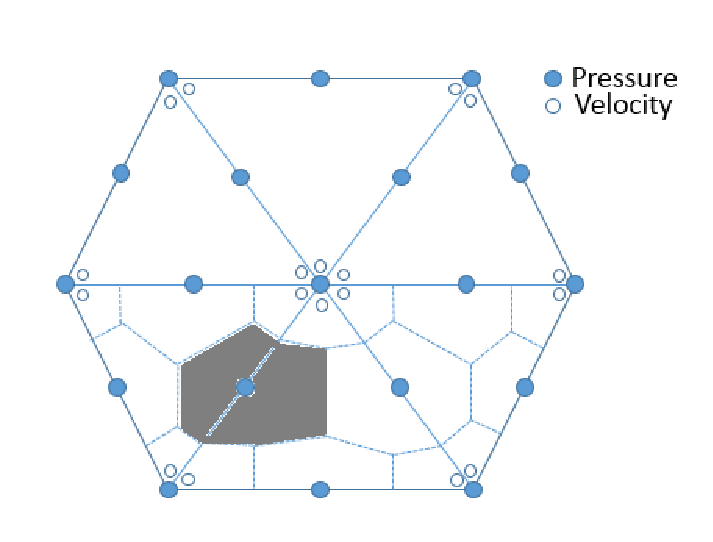
\includegraphics[width=.5\textwidth]{./Pics/P1DGP2.pdf}}
\caption{2D representation of \PN[1]{2} element pairs used in this work. Shaded areas denote control volumes across two contiguous elements. Blue and white circles represent pressure and velocity nodes, respectively.} 
\label{fig:fem_cv}
\end{figure}

\clearpage

%%%%
%%%%  FIGURE
%%%%
\begin{figure}[h]
\centering
\vbox{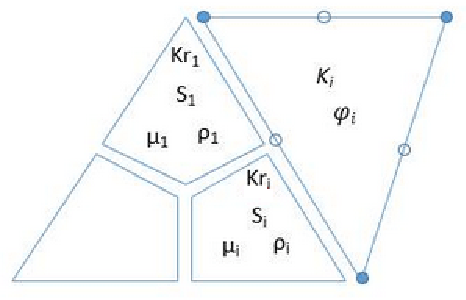
\includegraphics[width=.75\textwidth]{./Pics/element_n.pdf}}
\caption{This is a graphical representation of two different element types. Triangle {\it A} is a representation of the \PN[1]{2} element-pair, whereas triangle {\it B} represents the \PN[1]{1} element-pair. Porosity $\phi_{i}$, permeability {\bf K}$_{i}$, velocity and pressure are primarily represented in FE space whereas scalar fields (such as saturation, density, viscosity etc) are represented in CV space.}
\label{fig:fem_elem}
\end{figure}
\clearpage

%%%%
%%%%  FIGURE 
%%%%
\begin{figure}[h]
\centering
\vbox{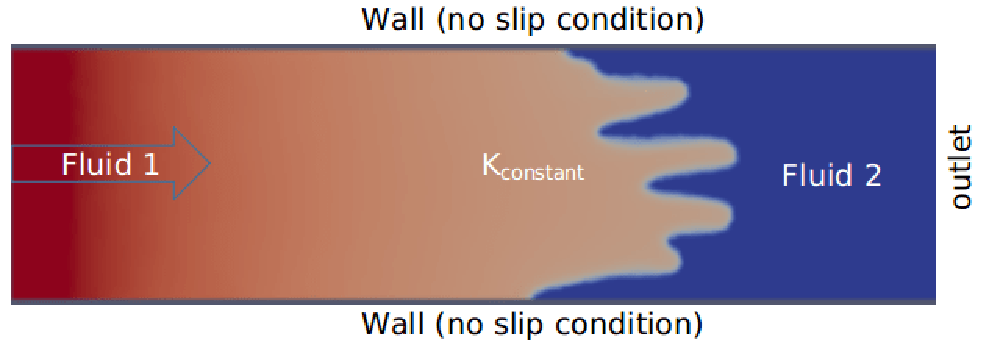
\includegraphics[width=0.75\textwidth]{./Pics/phase_vol_frac_uni_perm_1.pdf}}
\caption{Schematics of formation of flow instabilities during injection of a pure low viscosity fluid (red) into a domain saturated with a second fluid (dark blue). The ratio of viscosity between the two fluids is 5. In this case, the initially piston shape front collapses leading to the formation of several fingers.}
\label{fig:simple_case}
\end{figure}
\clearpage


%%%%
%%%%  FIGURE 
%%%%
\begin{figure}[ht] 
\vbox{
\hbox{\hspace{-0.3cm}
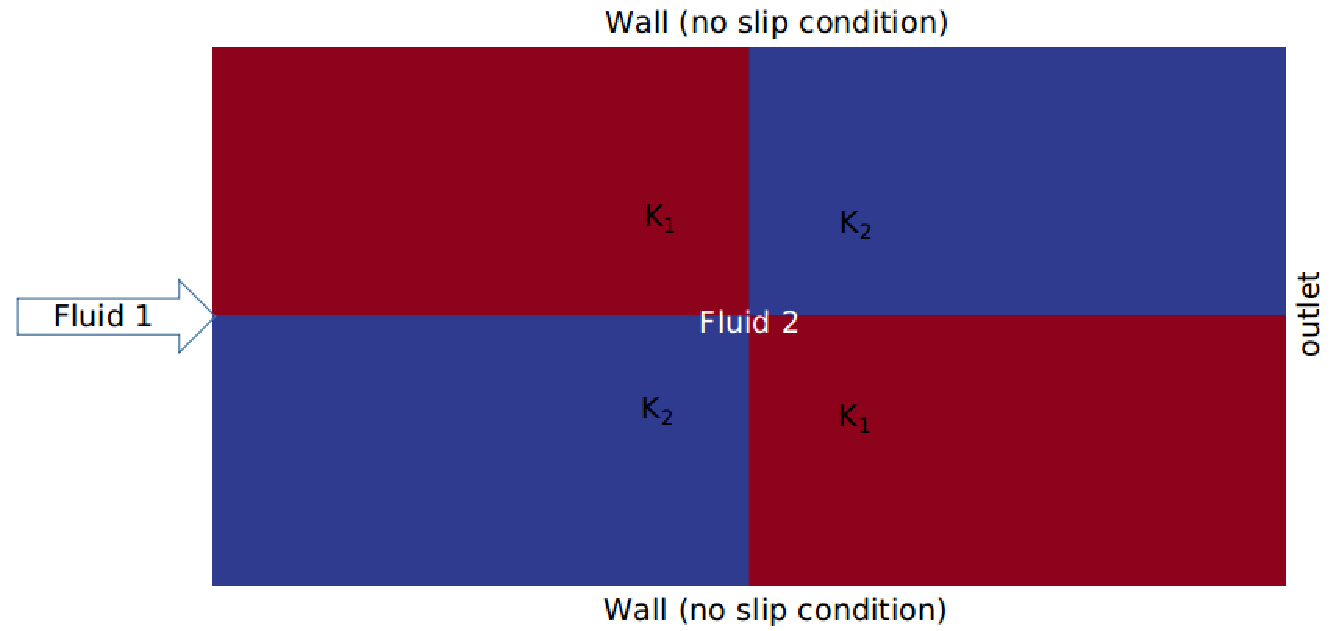
\includegraphics[width=.8\textwidth]{./Pics1/2b2_wi_fine/2b2_whole_in_fine_perm_1.pdf} 
}
\vspace{0.0cm}
\hbox{\hspace{3.5cm} (a) map of permeabilities ($\mathbf{K}$)
}
\vspace{0.25cm}
\hbox{\hspace{1.5cm}
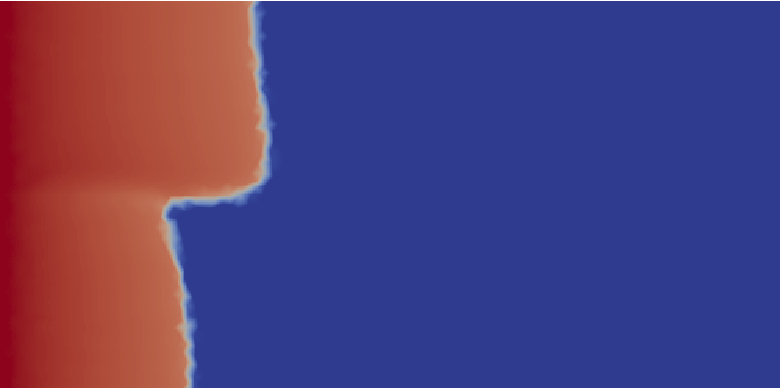
\includegraphics[width=.85\textwidth]{./Pics1/2b2_wi_fine/2b2_whole_in_fine_250_2.pdf}
}
\vspace{0.0cm}
\hbox{\hspace{4.5cm} (b) flow at t=250 
}
\vspace{0.25cm}
\hbox{\hspace{1.5cm}
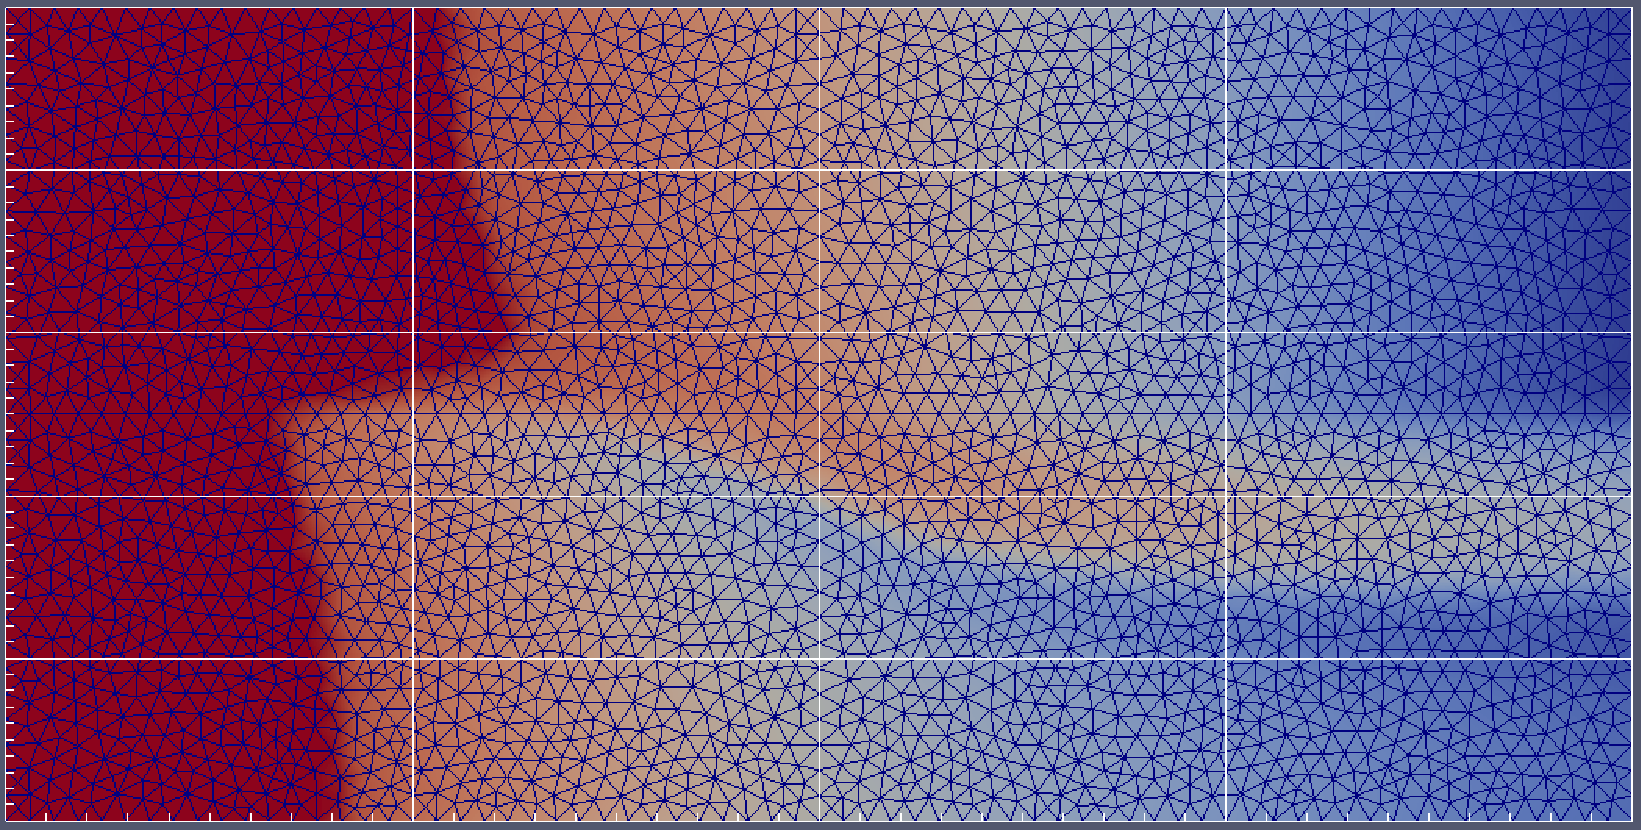
\includegraphics[width=.65\textwidth]{./Pics1/2b2_wi_fine/2b2_whole_in_fine_3000_2.pdf}
}
\vspace{0.0cm}
\hbox{\hspace{4.0cm} (c) flow at t=3000   
}}     
\caption{Model validation of fluid displacement in heterogeneous porous media ({\it VR}=1): (a) the domain is divided into four subdomains with prescribed synthetic permeability, $\mathbf{K}_{1}=1$ and $\mathbf{K}_{2}=2.5$; (b-c) snapshots of saturation (displacing fluid) field at t=$25$s and t=$300$ sec. The domain is discretised with $5960$ \PN[1]{2} elements. }
\label{fem_cv_represent_a}
\end{figure}
\clearpage



%%%%
%%%%  FIGURE
%%%%
\begin{landscape}
\begin{figure}[ht] 
\vbox{\vspace{-1cm}
\hbox{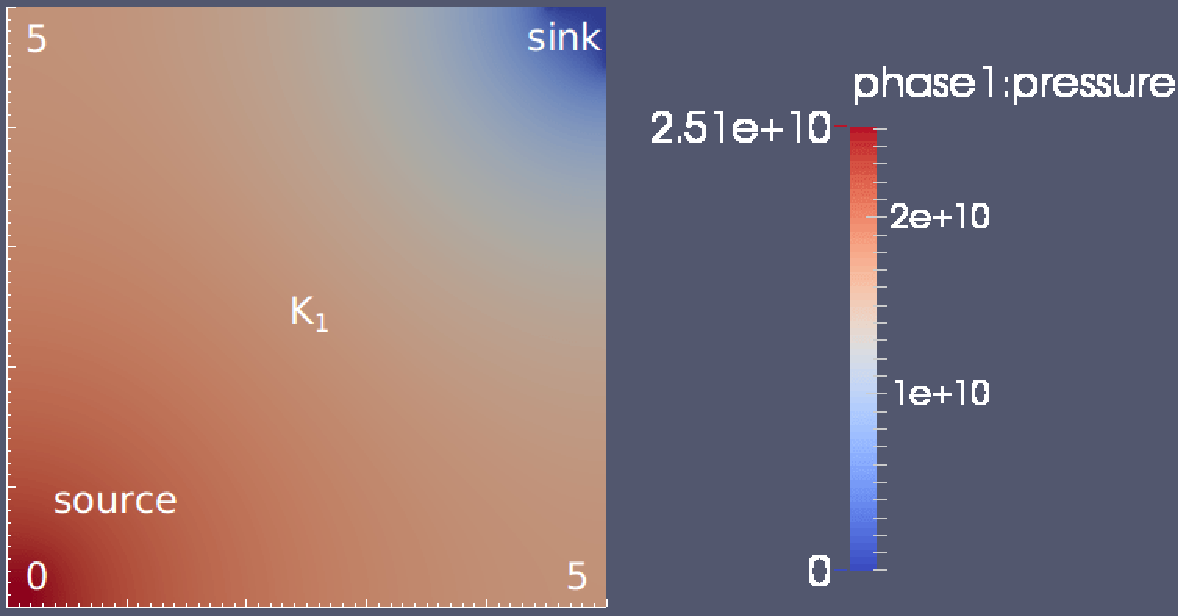
\includegraphics[width=.7\textwidth]{./Pics1/Saffman_homogeneous_MR3/saffman_homo_fixed_2.pdf}
      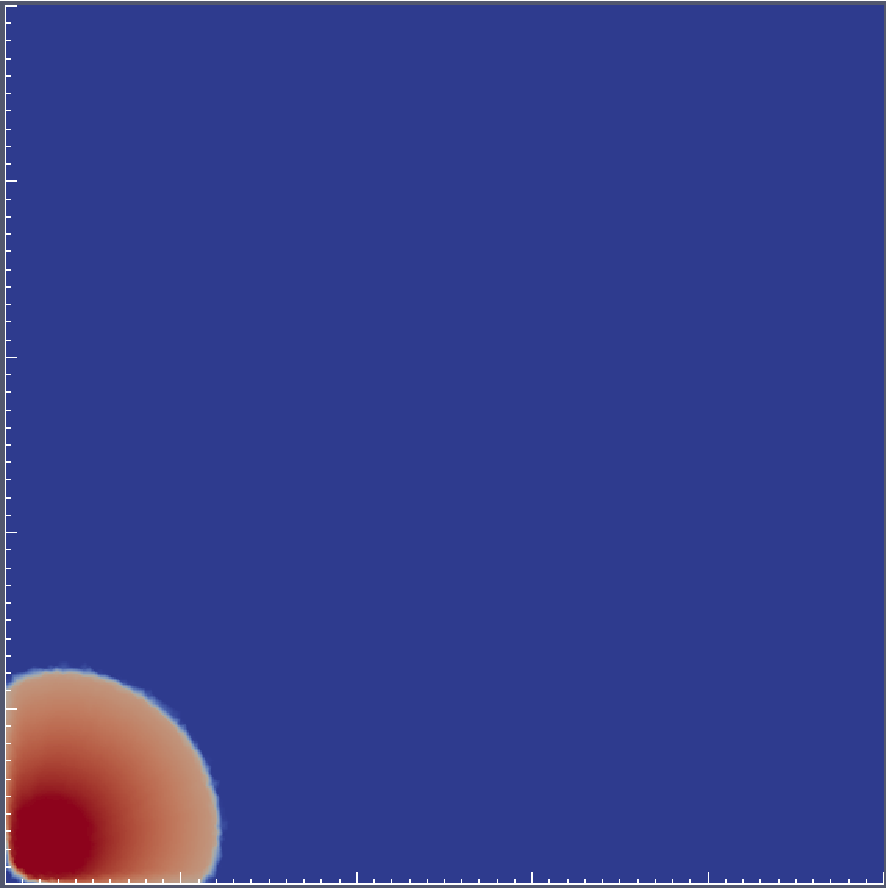
\includegraphics[width=.37\textwidth]{./Pics1/Saffman_homogeneous_MR3/saffman_homo_fixed_250.pdf}
      \includegraphics[width=.37\textwidth]{./Pics1/Saffman_homogeneous_MR3/saffman_homo_fixed_1000.pdf}}
\vspace{0.cm}
\hbox{\hspace{2.5cm} (a) pressure at t=0s \hspace{5.cm} (b) t=0.87s \hspace{2.75cm} (c) t=3.54s}
\vspace{0.5cm}
\hbox{
      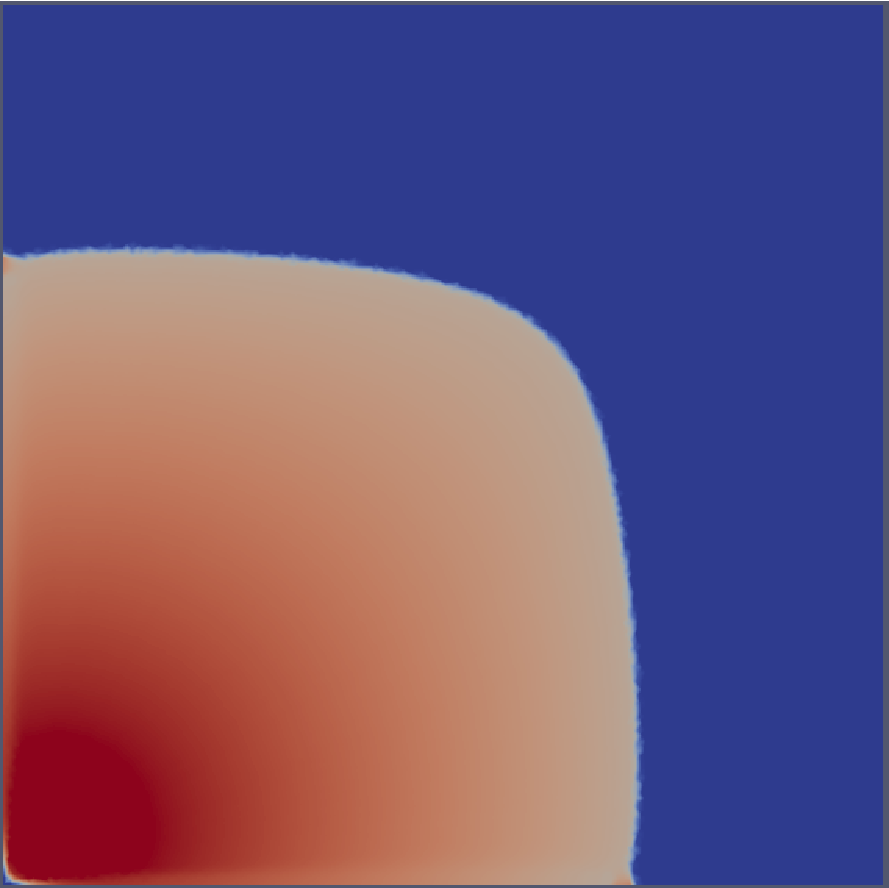
\includegraphics[width=.375\textwidth]{./Pics1/Saffman_homogeneous_MR3/saffman_homo_fixed_2500.pdf}
      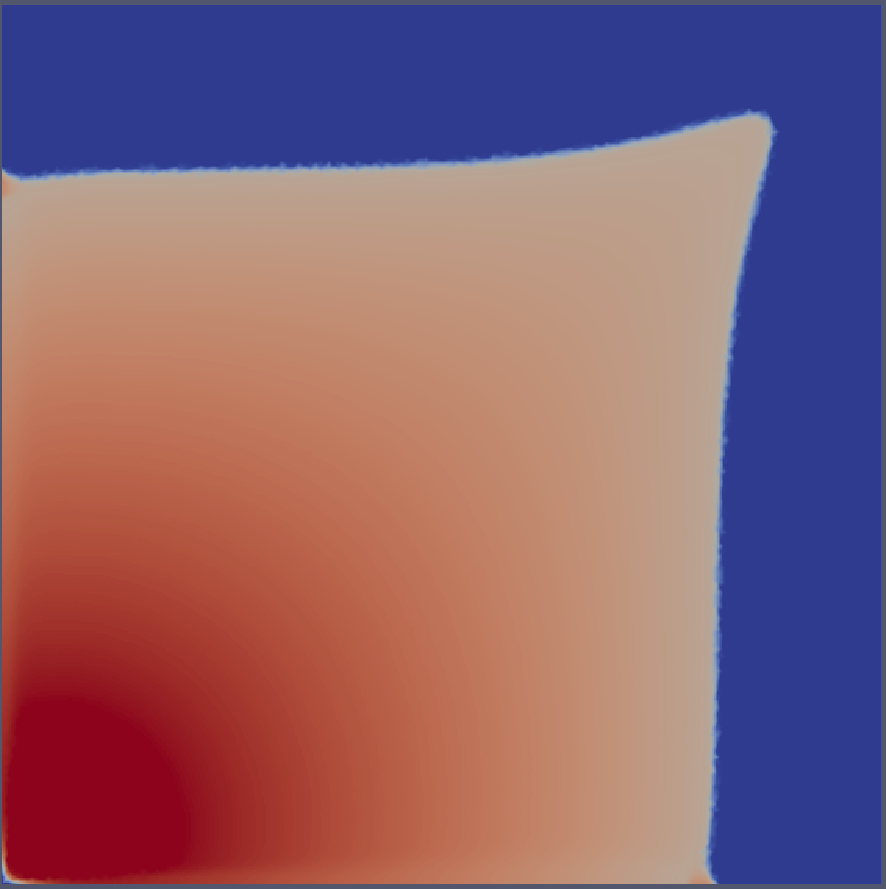
\includegraphics[width=.375\textwidth]{./Pics1/Saffman_homogeneous_MR3/saffman_homo_fixed_3500.pdf} 
      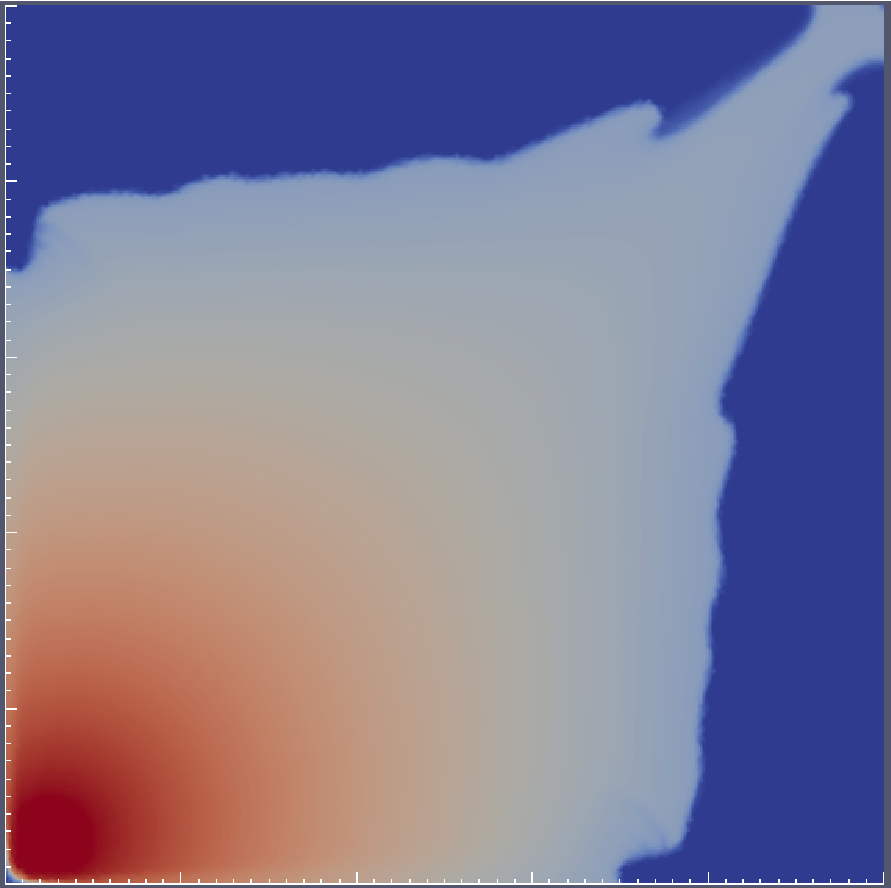
\includegraphics[width=.65\textwidth]{./Pics1/Saffman_homogeneous_MR3/saffman_homo_fixed_end.pdf}}
\vspace{0.cm}
\hbox{ \hspace{1.cm} (d) t=8.86s \hspace{3.0cm} (e) t=12.41s   \hspace{4.0cm} (f) t=17.95s}
\vspace{0.cm}
}   
\caption{Simulated flow in a Hele-Shaw cell ({\it VR}=3): (a) initial pressure profile $\left(\text{in g.cm}^{-1}\text{.s}^{-2}\right)$ with source and sink regions are explicitly shown along with dimensions (in cm); (b-f) snapshots of wetting phase saturation showing flow profile as the simulation evolves. The domain contains $47500$ \PN[1]{2} triangular elements.}
\label{fig:homoheleshaw_VN3}
\end{figure}
\end{landscape}
\clearpage



%%%%
%%%%  FIGURE
%%%%
\begin{landscape}
\begin{figure}[ht] 
\vbox{\vspace{-1cm}
\hbox{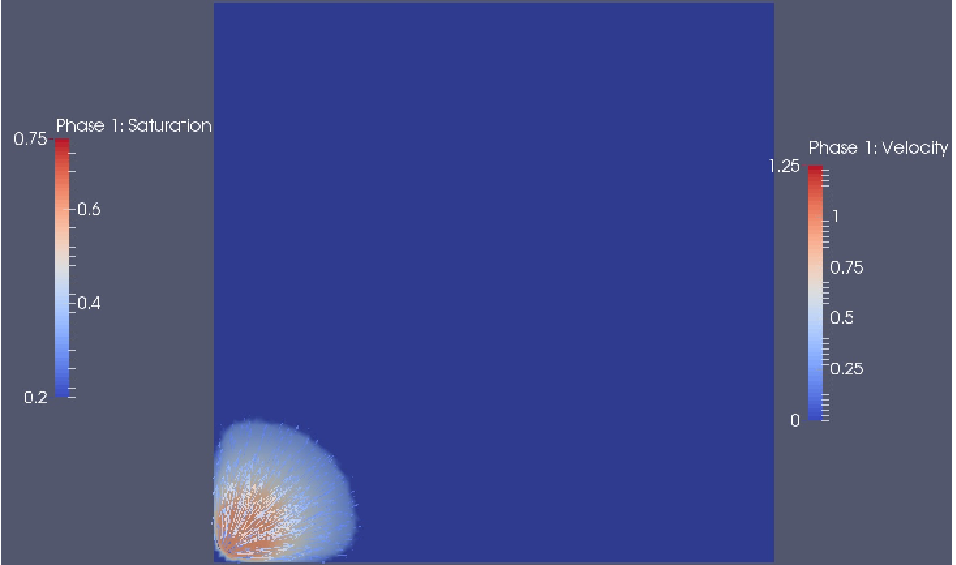
\includegraphics[width=.9\textwidth, height=0.5\textwidth]{./Pics1/Saffman_homogeneous_VR10/ST_Homog_VR10_D201c.pdf}
\hspace{0.5cm}      
      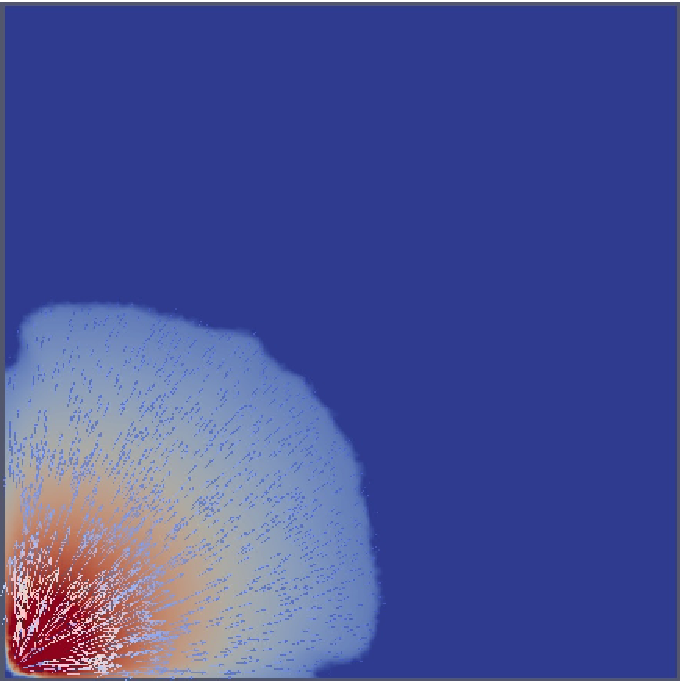
\includegraphics[width=.5\textwidth]{./Pics1/Saffman_homogeneous_VR10/ST_Homog_VR10_D1001c.pdf}}
\vspace{0.cm}
\hbox{\hspace{5.cm} (a) t=0.66s \hspace{8.cm} (b) t=3.43s }
\vspace{0.5cm}
\hbox{
      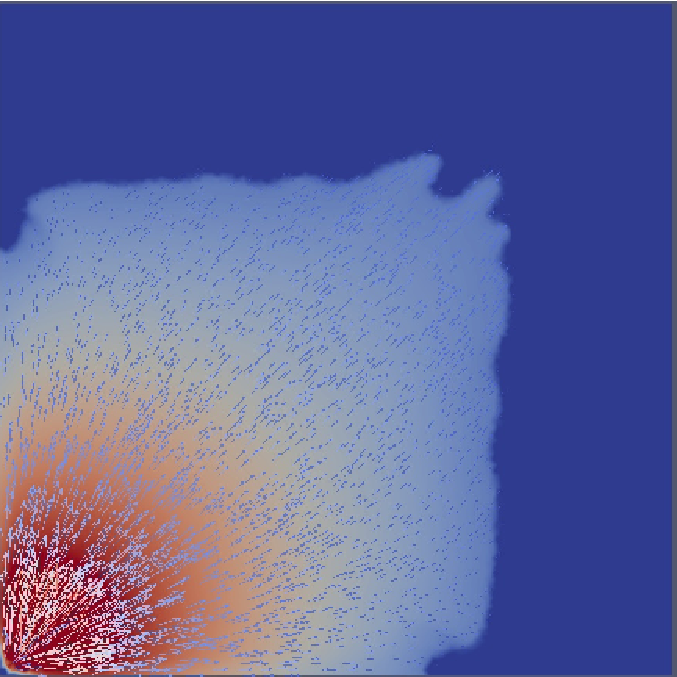
\includegraphics[width=.5\textwidth]{./Pics1/Saffman_homogeneous_VR10/ST_Homog_VR10_D2001c}
      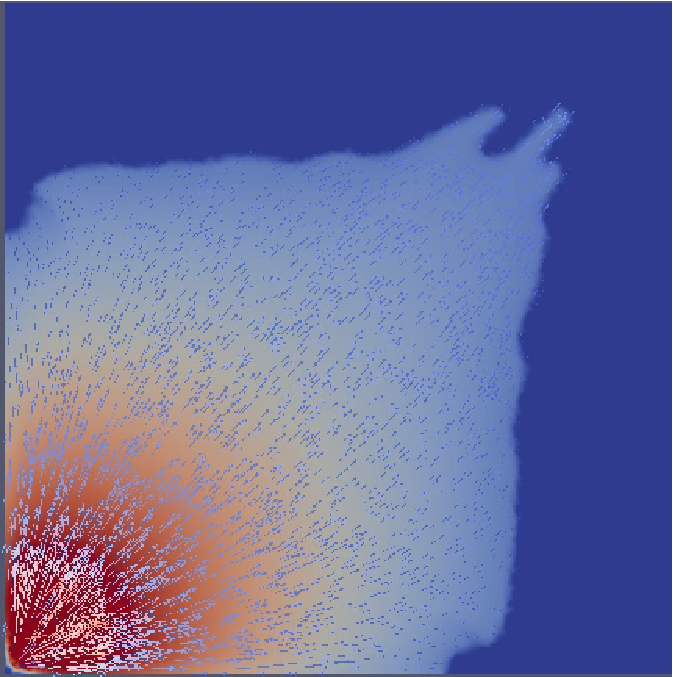
\includegraphics[width=.5\textwidth]{./Pics1/Saffman_homogeneous_VR10/ST_Homog_VR10_D2201c}
      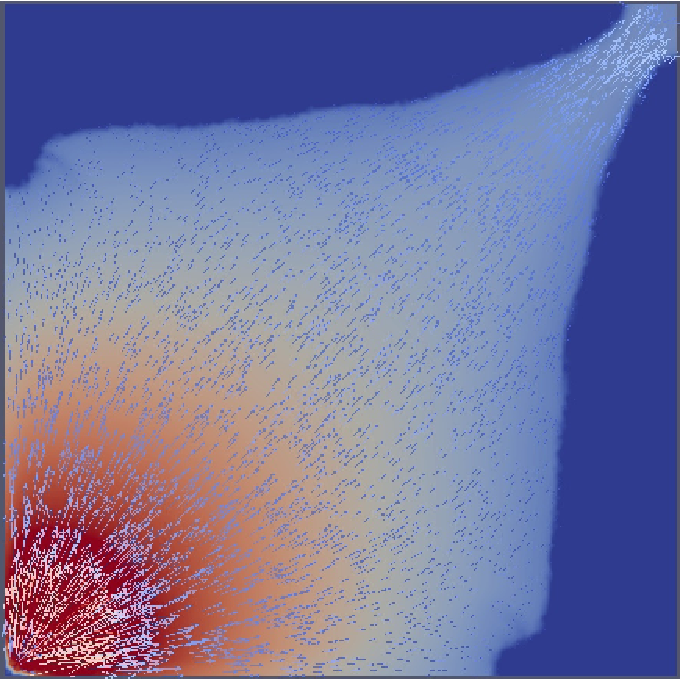
\includegraphics[width=.5\textwidth]{./Pics1/Saffman_homogeneous_VR10/ST_Homog_VR10_D3001c}}
\vspace{0.cm}
\hbox{ \hspace{2.cm} (c) t=6.92s \hspace{4.5cm} (d) t=7.61s \hspace{4.5cm} (e)t=10.00s}
\vspace{0.cm}
}   
\caption{Simulated flow in a Hele-Shaw cell ({\it VR}=10): snapshots of overlapped wetting phase saturation and velocity vectors showing flow profile as the simulation evolves. The domain contains $26313$ \PN[1]{2} triangular elements.}
\label{fig:homoheleshaw_VN10}
\end{figure}
\end{landscape}
\clearpage

%%%%
%%%%  FIGURE
%%%%
\begin{landscape}
\begin{figure}[ht] 
\vbox{\vspace{-1cm}
\hbox{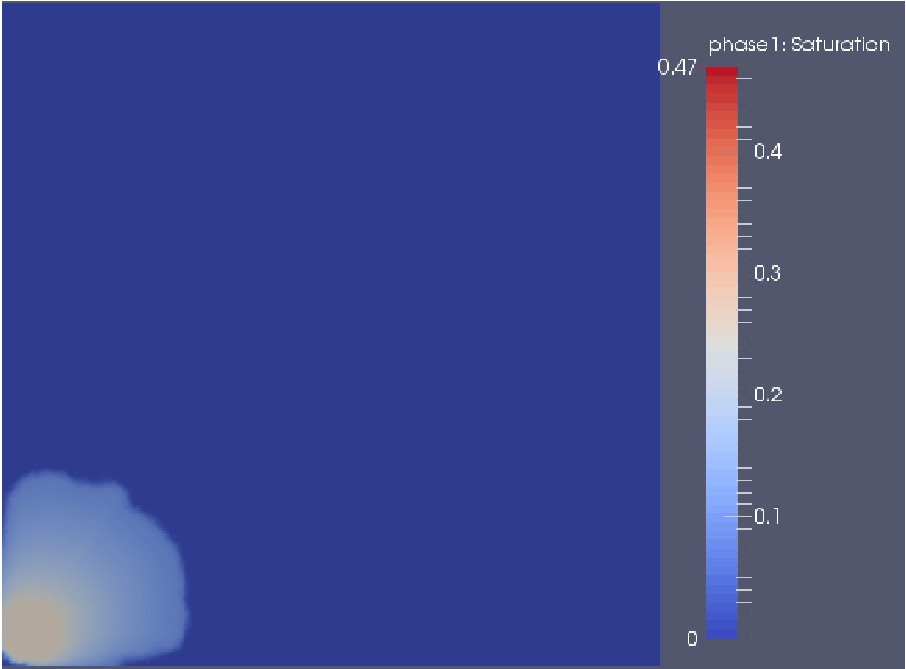
\includegraphics[width=.9\textwidth, height=0.5\textwidth]{./Pics1/Saffman_homogeneous_VR150/ST_Homog_VR150_D300b}
\hspace{0.5cm}      
      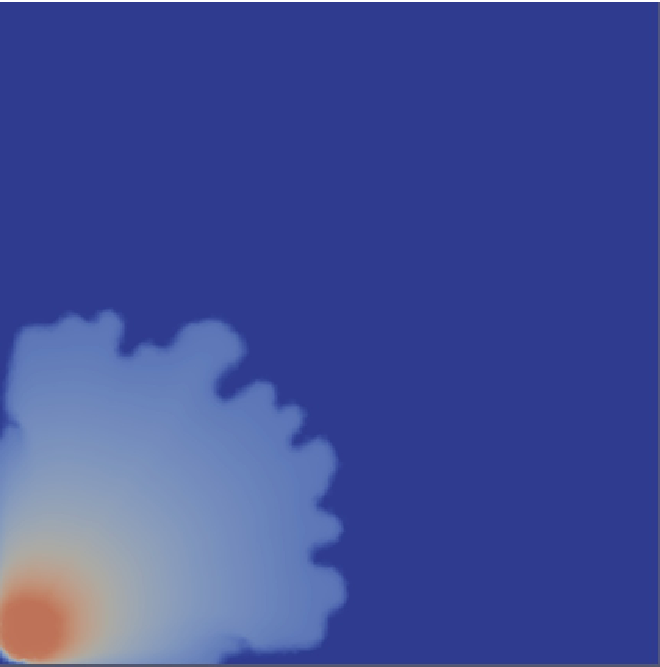
\includegraphics[width=.5\textwidth]{./Pics1/Saffman_homogeneous_VR150/ST_Homog_VR150_D1600b}}
\vspace{0.cm}
\hbox{\hspace{5.cm} (a) t=0.27s \hspace{8.cm} (b) t=0.94s }
\vspace{0.5cm}
\hbox{
      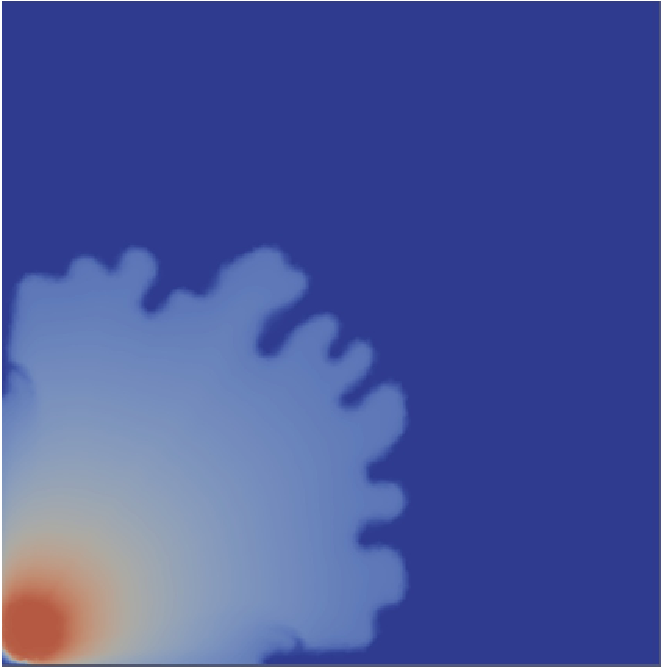
\includegraphics[width=.5\textwidth]{./Pics1/Saffman_homogeneous_VR150/ST_Homog_VR150_D2700b}
      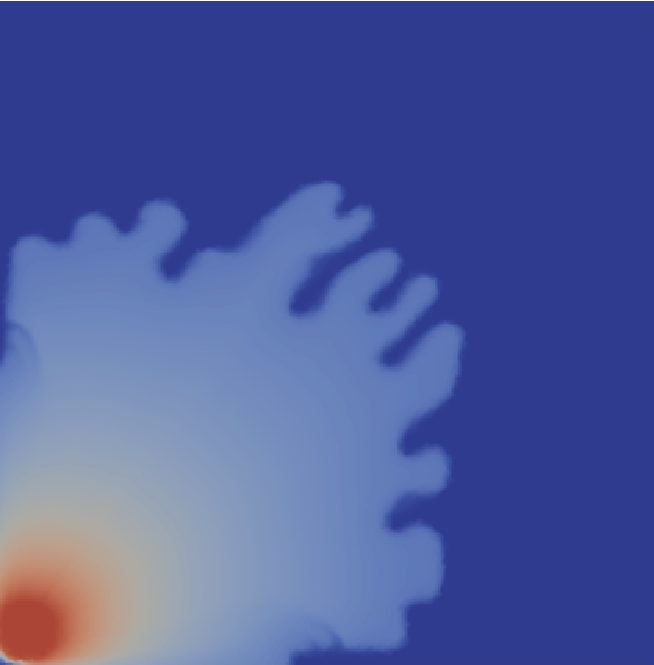
\includegraphics[width=.5\textwidth]{./Pics1/Saffman_homogeneous_VR150/ST_Homog_VR150_D4000b}
      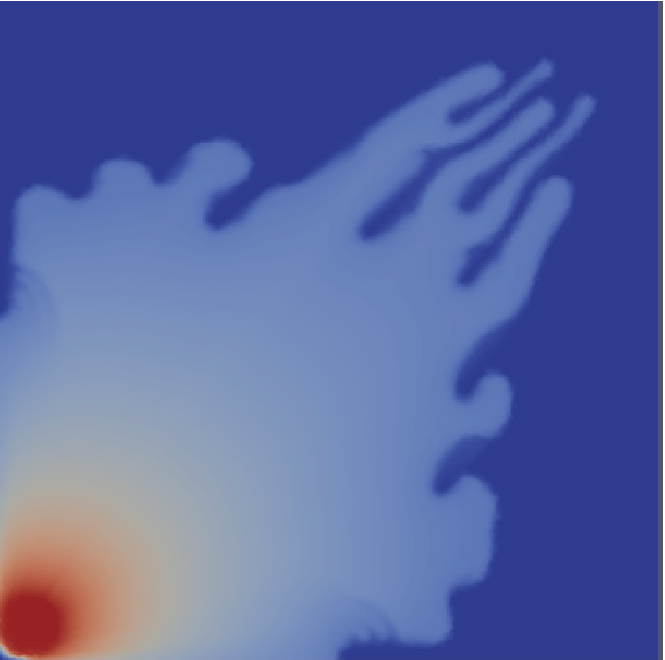
\includegraphics[width=.5\textwidth]{./Pics1/Saffman_homogeneous_VR150/ST_Homog_VR150_D7000b}}
\vspace{0.cm}
\hbox{ \hspace{2.cm} (c) t=1.32s \hspace{4.5cm} (d) t=1.70s \hspace{4.5cm} (e)t=2.31s}
\vspace{0.cm}
}   
\caption{Simulated flow in a Hele-Shaw cell ({\it VR}=150): snapshots of wetting phase saturation showing flow profile as the simulation evolves. The domain contains $26313$ \PN[1]{2} triangular elements.}
\label{fig:homoheleshaw_VN10}
\end{figure}
\end{landscape}
\clearpage


%%%%
%%%%  FIGURE
%%%%
\begin{landscape}
\begin{figure}[ht] 
\hbox{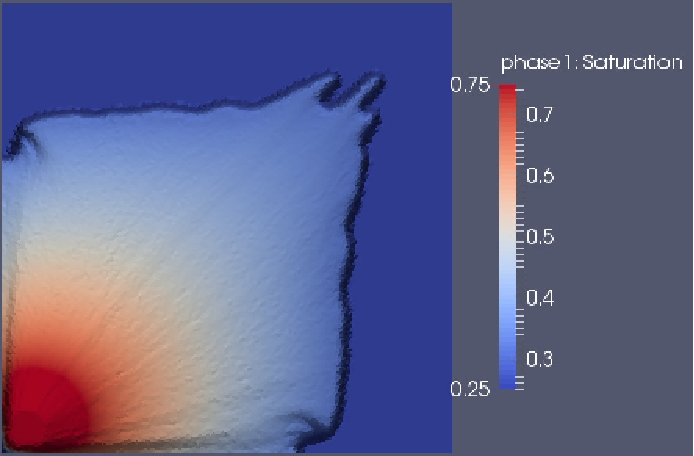
\includegraphics[width=.5\textwidth]{./Pics1/Saffman_homogeneous_VR10/ST_Homog_VR10_D2201_bbd}
       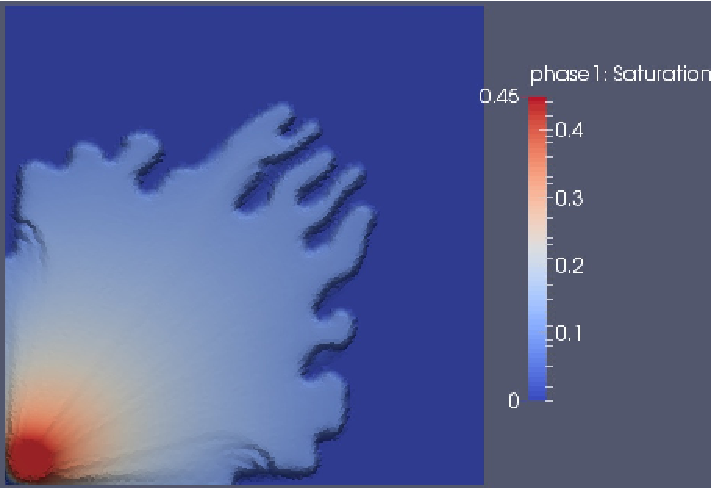
\includegraphics[width=.49\textwidth]{./Pics1/Saffman_homogeneous_VR150/ST_Homog_VR150_D5003_k2b}}
\caption{Simulated flow in Hele-Shaw cells performed with viscosity ratios of 10 (left, t=7.61s) and 150 (t=1.94s). Width of largest fingers are approximetely 0.70 and 0.90cm, which are in good agreement with values obtained from \citet{guan_2003}'s analytic solution. Domains of both simulations contain $26313$ \PN[1]{2} triangular elements.\red{(More pics to be added!!)}}
\label{fig:homoheleshaw_VN10_VN150}
\end{figure}
\end{landscape}



\begin{comment}

%%%%
%%%%  FIGURE
%%%%
\begin{landscape}
\begin{figure}[ht] 
\vbox{\vspace{-1cm}
\hbox{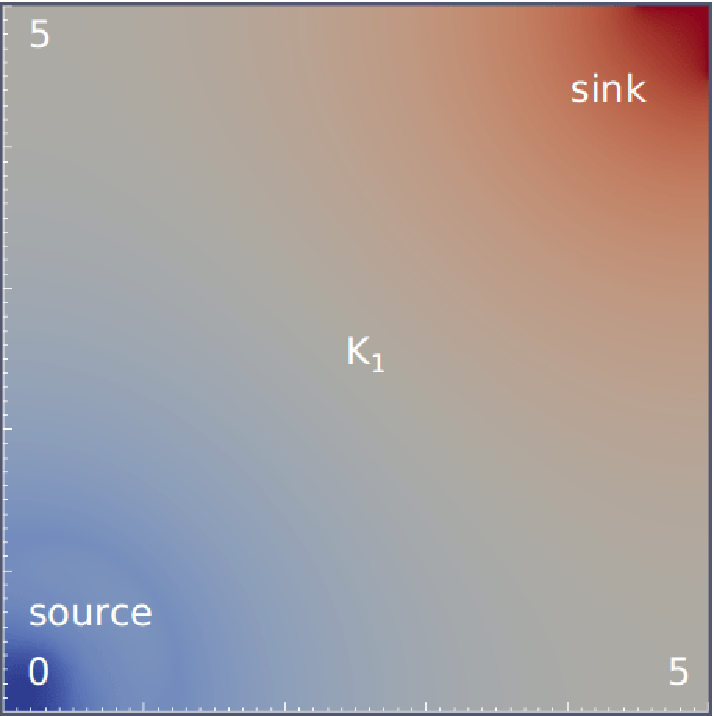
\includegraphics[width=.5\textwidth]{./Pics1/Saffman_homogeneous/saffman_homo_fixed_1.pdf}
      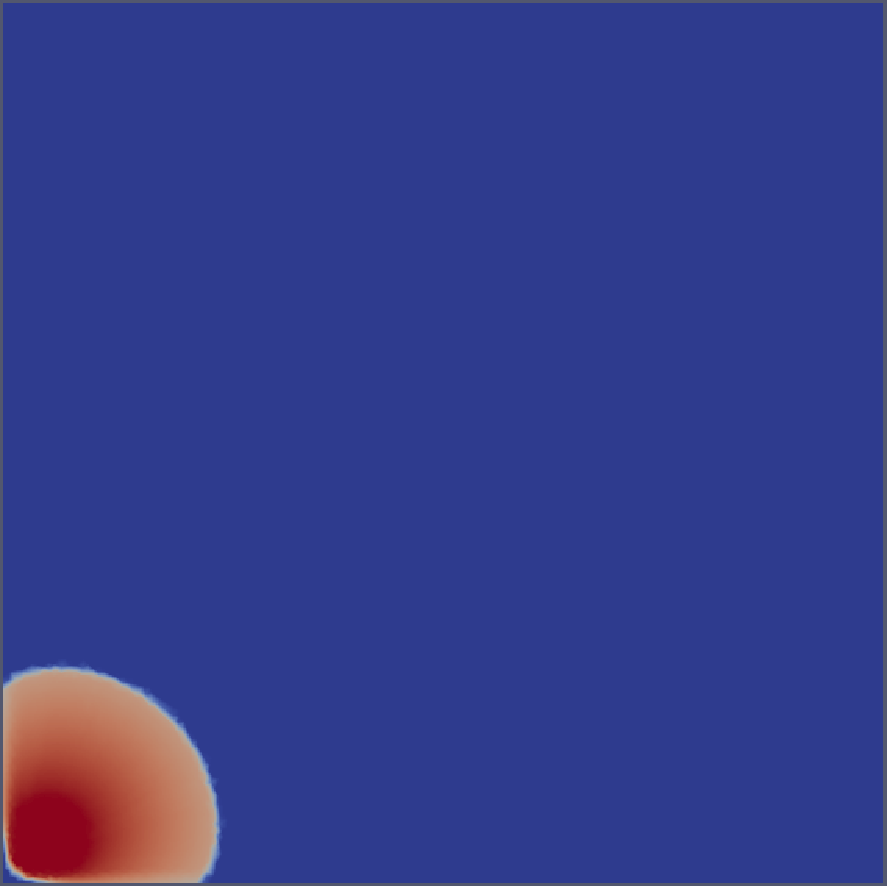
\includegraphics[width=.5\textwidth]{./Pics1/Saffman_homogeneous/saffman_homo_fixed_250_1.pdf}
      \includegraphics[width=.5\textwidth]{./Pics1/Saffman_homogeneous/saffman_homo_fixed_1000.pdf}}
\vspace{0.cm}
\hbox{\hspace{1.0cm} (a) pressure at t=0 \hspace{3.cm} (b) t=250\red{(???)} \hspace{3.0cm} (c) t=1000\red{(???)}}
\vspace{0.5cm}
\hbox{
      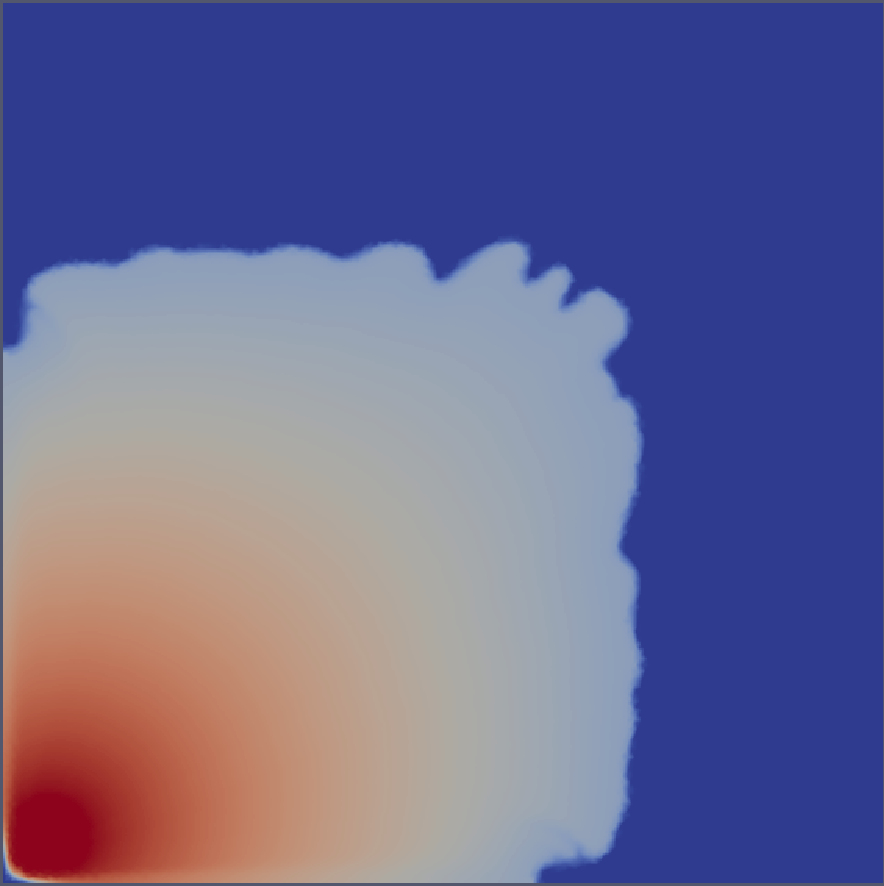
\includegraphics[width=.5\textwidth]{./Pics1/Saffman_homogeneous/saffman_homo_fixed_6000.pdf}
      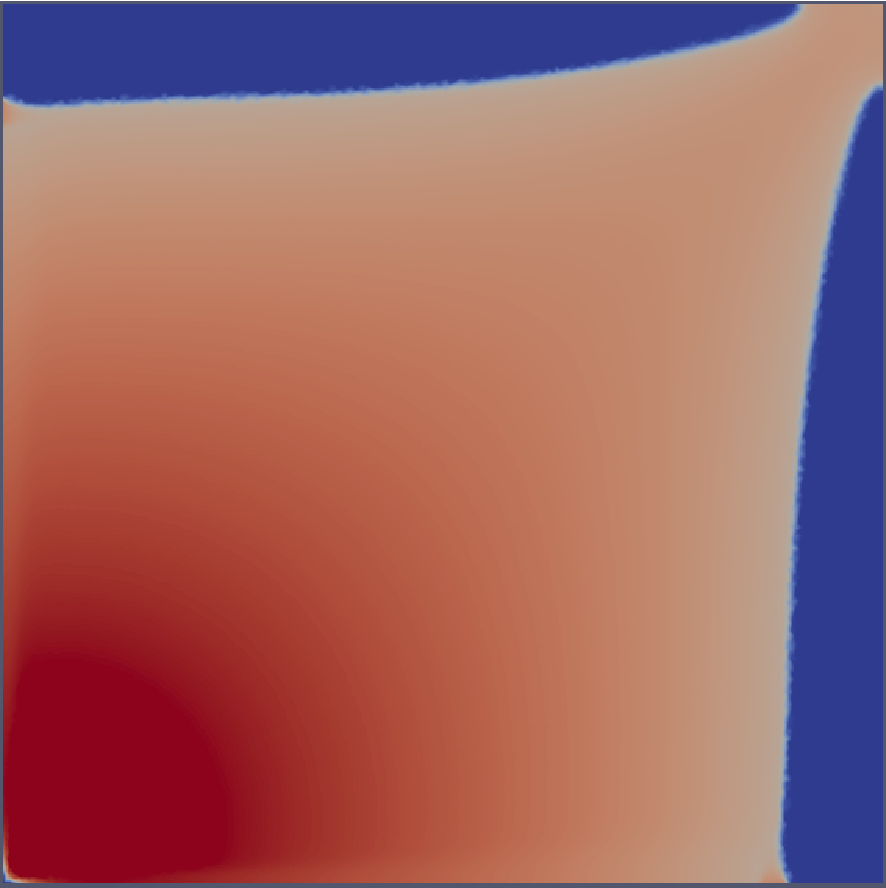
\includegraphics[width=.5\textwidth]{./Pics1/Saffman_homogeneous/saffman_homo_fixed_end_1.pdf}}
\vspace{0.cm}
\hbox{ \hspace{2.cm} (d) t=6000\red{(???)} \hspace{3.cm} (e) t=XXX\red{(???)}}
\vspace{0.cm}
}   
\caption{Simulated flow in a Hele-Shaw cell ({\it VR}=10): (a) pressure profile $\left(\text{in g.cm}^{-1}\text{.s}^{-2}\right)$ with source and sink regions explicitly shown along with dimensions (in cm); (b-e) snapshots of wetting phase saturation showing flow profile as the simulation evolves. The domain contains $47000$ \PN[1]{2} triangular elements. The pressure and saturation range of values are the same like the  case in fig.\ref{fig:homoheleshaw_VN3}.}
\label{fig:homoheleshaw_VN10}
\end{figure}
\end{landscape}
\clearpage
\end{comment}


%%%
%%% FIGURE XXXXXX
%%%
\begin{landscape}
  \begin{figure}[ht]
  \vbox{\vspace{-1cm}
      \hbox{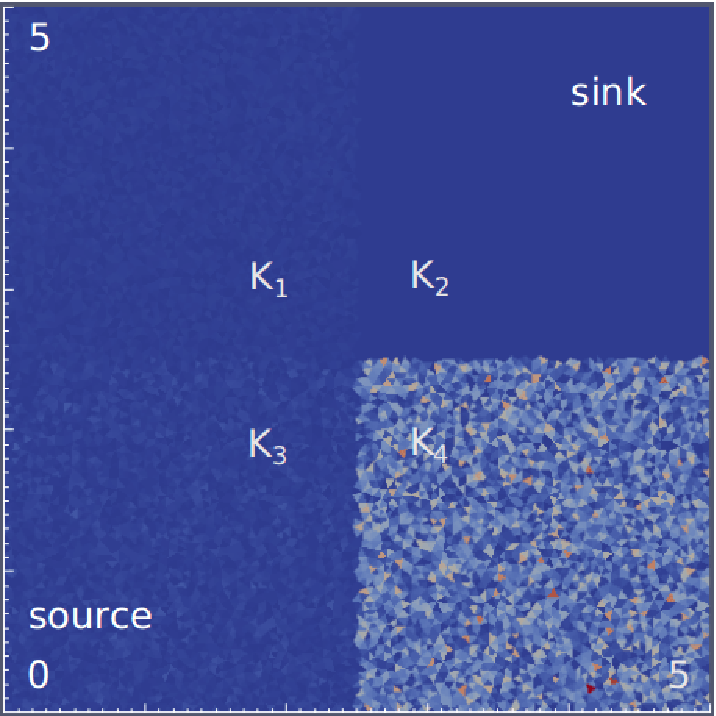
\includegraphics[width=.5\textwidth]{./Pics1/Saffman_heterogeneous/saffman_heter_fixed_1.pdf}
            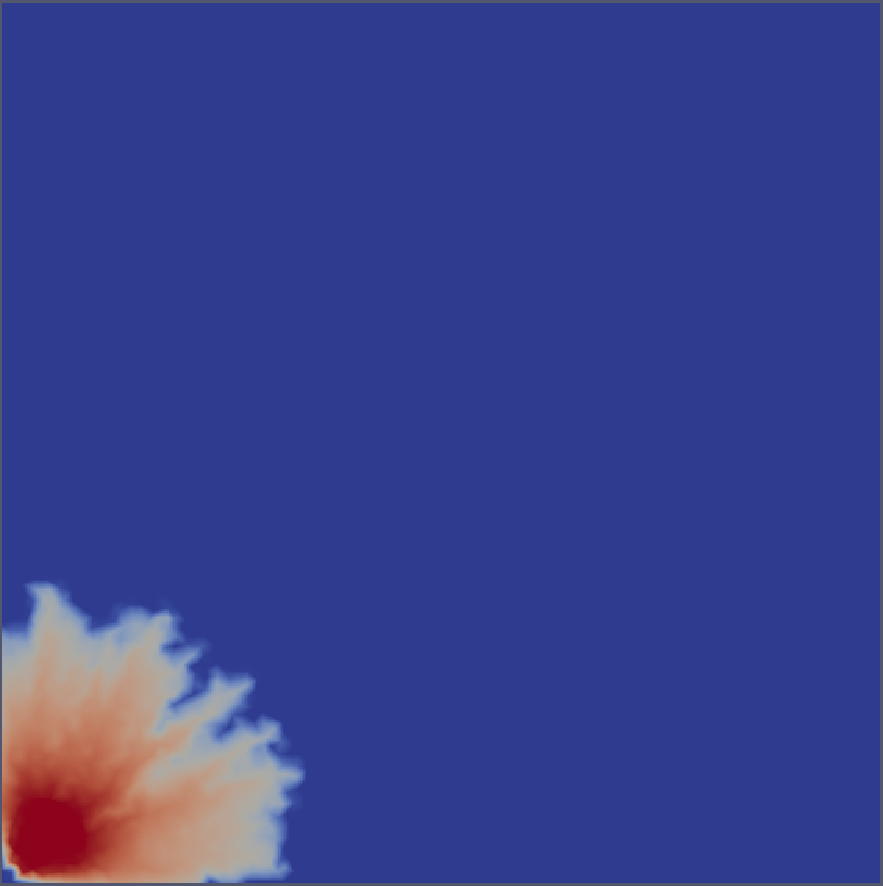
\includegraphics[width=.5\textwidth]{./Pics1/Saffman_heterogeneous/saffman_heter_fixed_500.pdf} 
            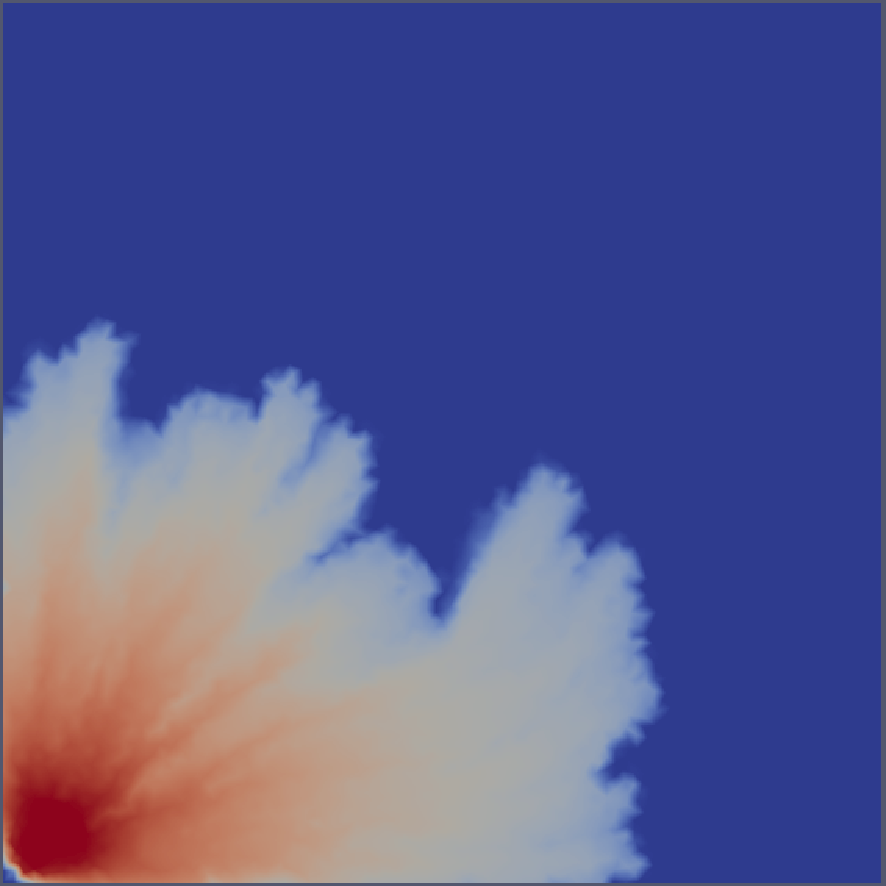
\includegraphics[width=.5\textwidth]{./Pics1/Saffman_heterogeneous/saffman_heter_fixed_2000.pdf} }
      \hbox{\hspace{1.0cm} (a) permeability map \hspace{3.cm} (b) t=0.75s \hspace{4.0cm} (c) t=8s}
      \vspace{0.5cm}
      \hbox{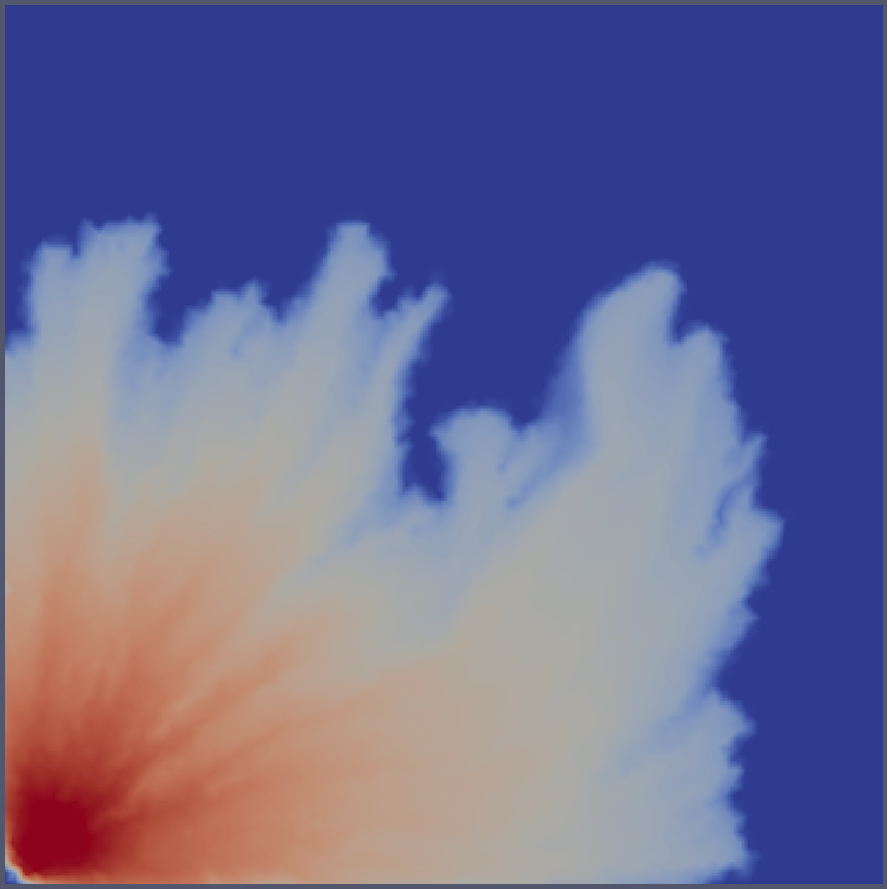
\includegraphics[width=.5\textwidth]{./Pics1/Saffman_heterogeneous/saffman_heter_fixed_3000.pdf}
            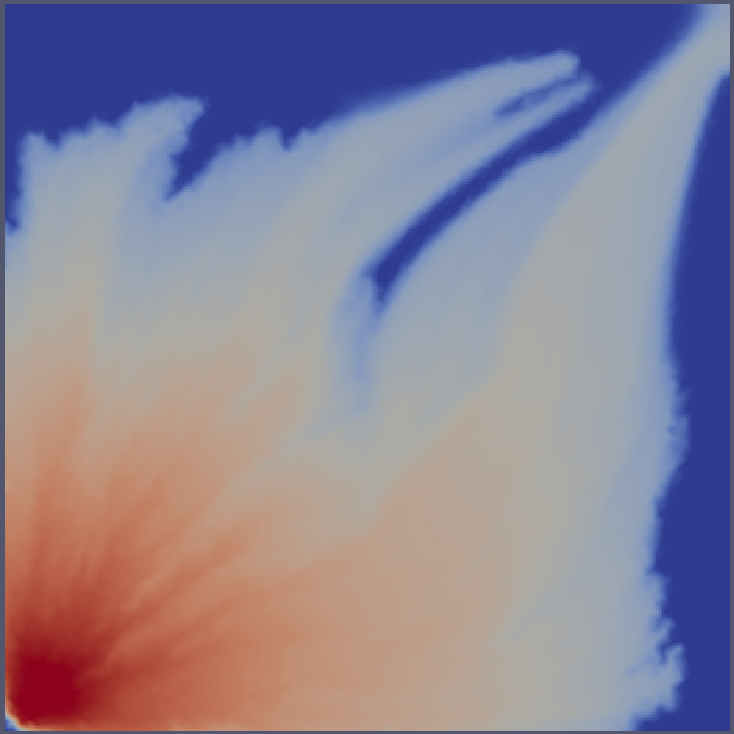
\includegraphics[width=.5\textwidth]{./Pics1/Saffman_heterogeneous/saffman_heter_fixed_6000.pdf}
            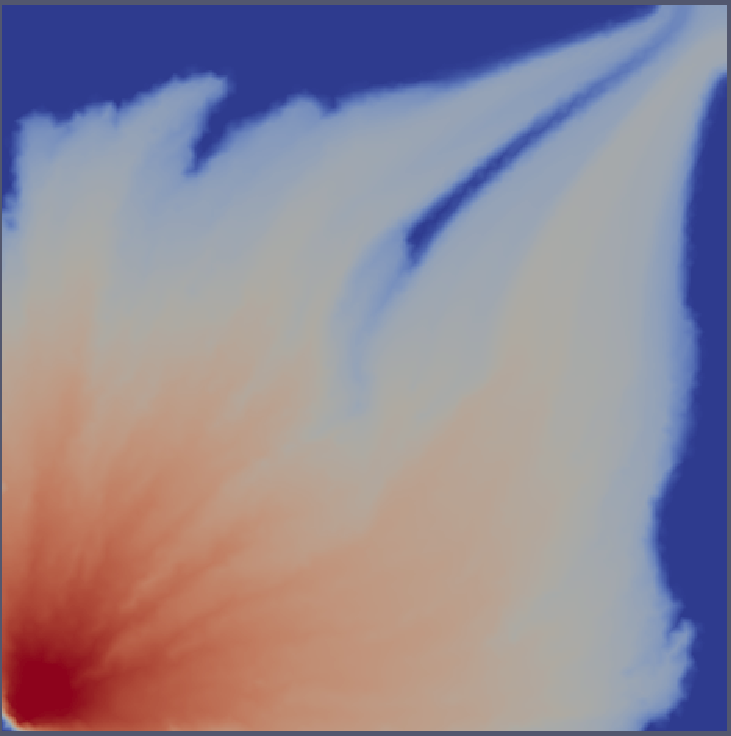
\includegraphics[width=.5\textwidth]{./Pics1/Saffman_heterogeneous/saffman_heter_fixed_24000.pdf} }
      \hbox{\hspace{2.5cm} (d) t=18s \hspace{5.cm} (e) t= \hspace{3.0cm} (f) t=24000 }}
\caption{Simulated flow in a modified Hele-Shaw cell with {\it VR}=10: (a) permeability distribution $\left(\text{10}^{-10}\le\mathbf{K}_{1}\le\text{5}\times\text{10}^{-10}\right.$, {\bf K}$_{2}$=10$^{-10}$, 10$^{-11}\le\mathbf{K}_{3}\le$ 5$\times$10$^{-10}$ and 10$^{-12}\le\mathbf{K}_{4}\le$ 5$\times$10$\left.^{-10}\text{ cm}^{2}\right)$; (b-f) snapshots of saturation profile during \red{XX} seconds of simulation. The domain contains \red{XX} \PN[1]{2} element-pairs.}
\label{fig:HeleShawHeter_VR10}
\end{figure}
\end{landscape}
\clearpage



%%%%
%%%%  FIGURE
%%%%
\begin{landscape}
\begin{figure}[ht] 
\vbox{
\hbox{\hspace{4.0cm}
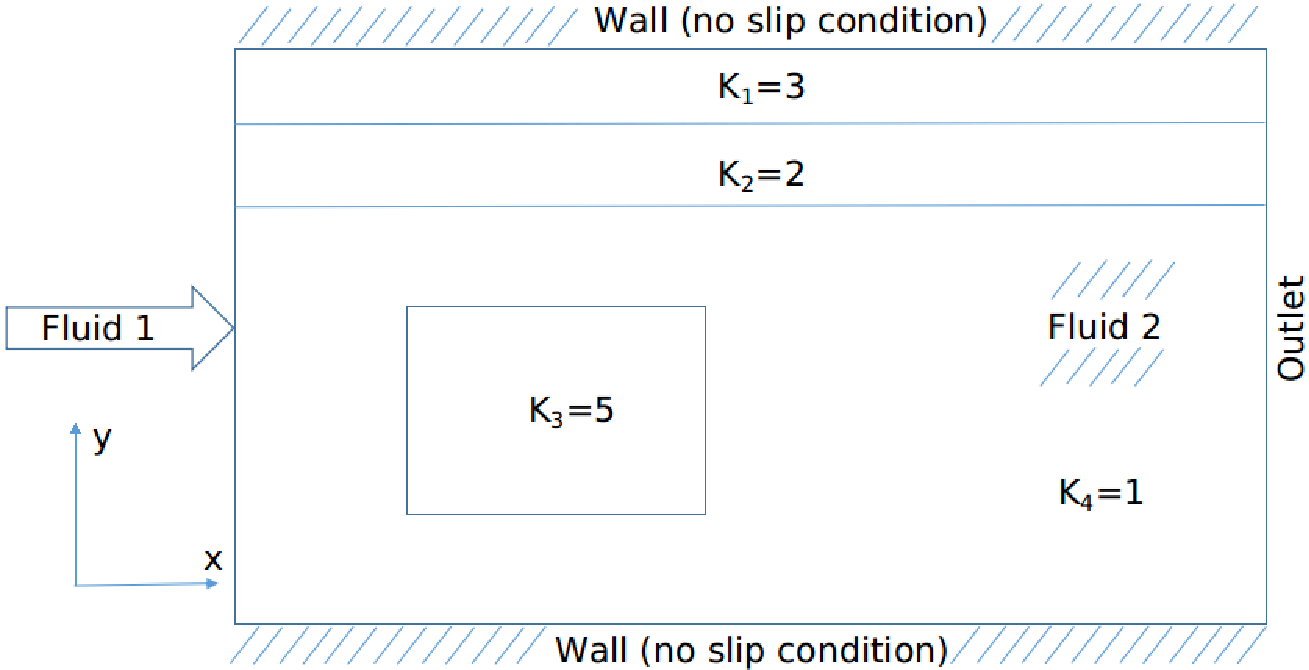
\includegraphics[width=.75\textwidth]{./Pics/map_of_boundaries.pdf} 
}
\vspace{0.0cm}
\hbox{\hspace{6.5cm} (a) map of permeabilties K   
}
\vspace{0.25cm}
\hbox{\hspace{4.0cm}
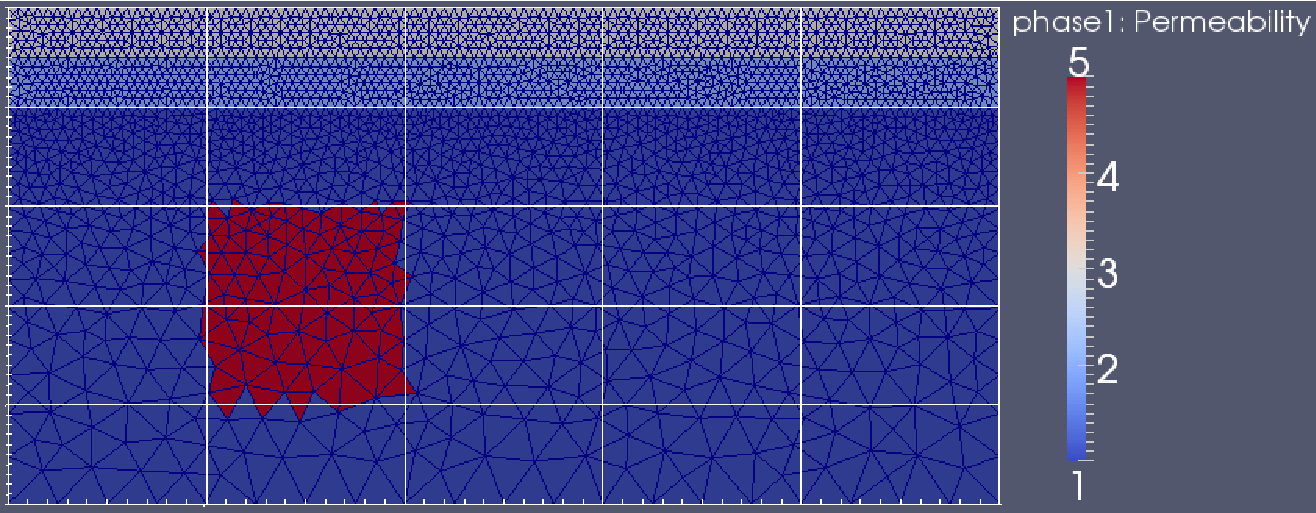
\includegraphics[width=.9\textwidth]{./Pics/map_of_boundaries_1.pdf}
}
\vspace{0.0cm}
\hbox{\hspace{9cm} (b)      
}
}     
\caption{Figure (a) describes the initial and boundary conditions as these are applied in this set of simulations. Below (b) there is a comparison between the unstructured and fixed mesh and the unstructured and adaptive mesh. During the implementation of fixed mesh initially there $4606$ elements while for the adaptive mesh there are $606$ while the majority of them is on the interface between between the two fluids. }
\label{fig:testcase_heter_domain}
\end{figure}
\end{landscape}
\clearpage



%%%%
%%%%  FIGURE
%%%%
\begin{landscape}
\begin{figure}[ht] 
\vbox{
\hbox{\hspace{3.5cm}
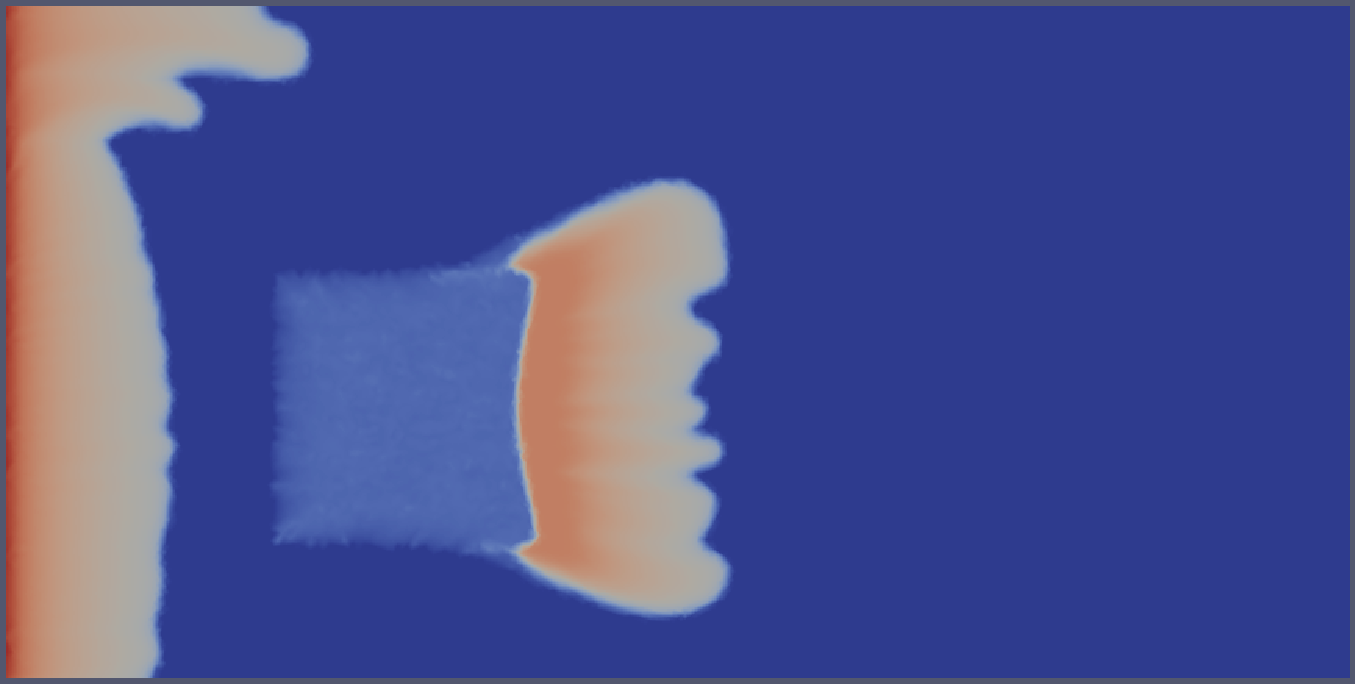
\includegraphics[width=.65\textwidth]{./Pics1/mr10_5regions_fixed/5regions_fixed_250.pdf} 
}
\vspace{0.0cm}
\hbox{\hspace{6.5cm} (a) flow at t=250 (fixed mesh)  
}
\vspace{0.25cm}
\hbox{\hspace{3.5cm}
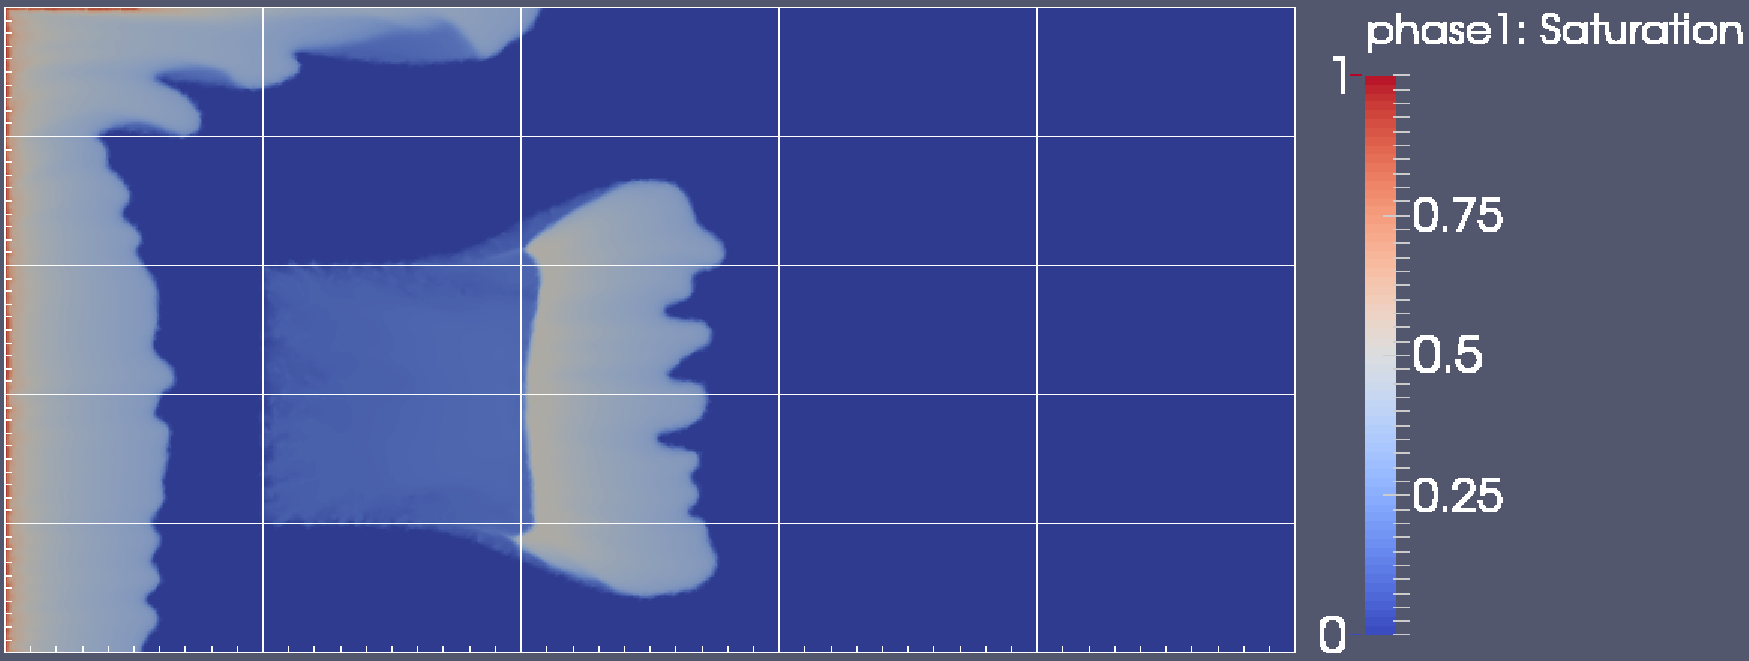
\includegraphics[width=.9\textwidth]{./Pics1/mr10_5regions_adapt/5regions_adapt_250_1.pdf}
}
\vspace{0.0cm}
\hbox{\hspace{6.5cm} (b) flow at t=250 (adaptive mesh)    
}
}     
\caption{For $t=0.125$s, $2$ test-cases under the VR=$10$ and under fixed (top) and adaptive(bottom) mesh are compared. There is a significant difference on the main front (left hand side of the domain) and the number of finger that appear.}
\label{fig:2testcase_a}
\end{figure}
\end{landscape}
\clearpage


%%%%
%%%%  FIGURE
%%%%
\begin{landscape}
\begin{figure}[ht] 
\vbox{
\hbox{\hspace{3.5cm}
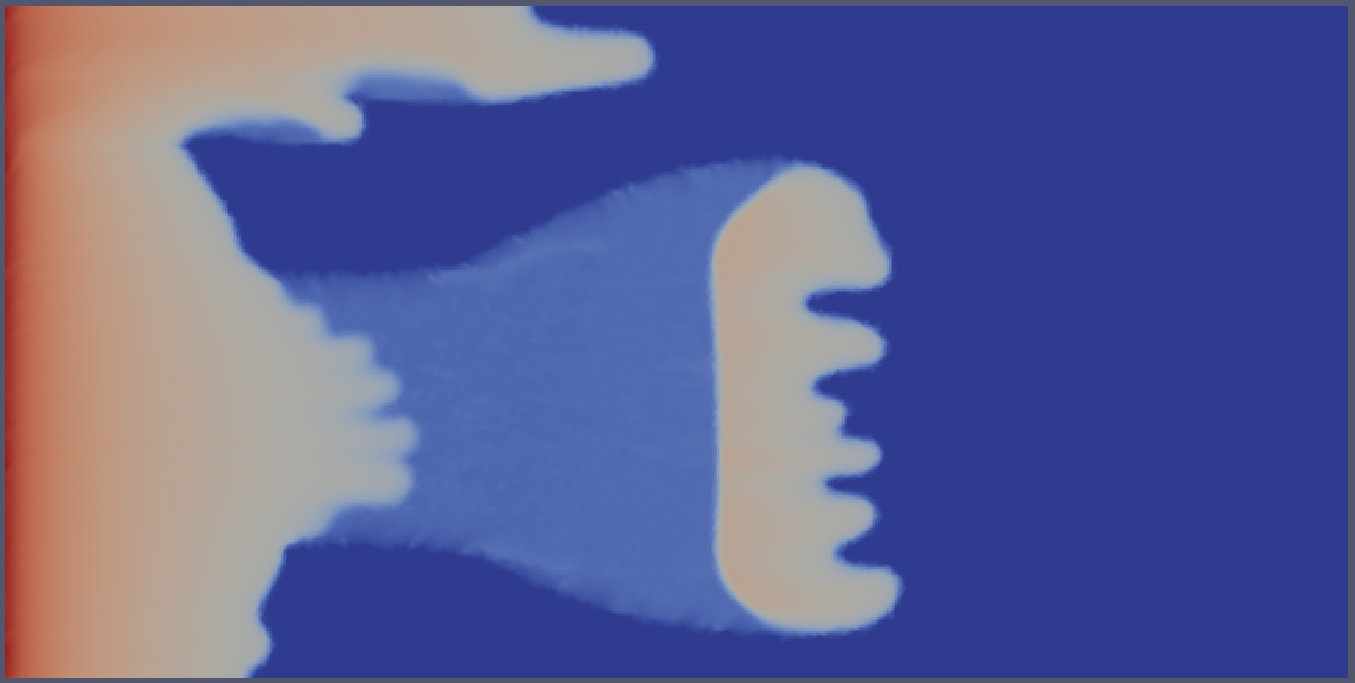
\includegraphics[width=.65\textwidth]{./Pics1/mr10_5regions_fixed/5regions_fixed_500.pdf} 
}
\vspace{0.0cm}
\hbox{\hspace{6.5cm} (a) flow at t=500 (fixed mesh)   
}
\vspace{0.25cm}
\hbox{\hspace{3.5cm}
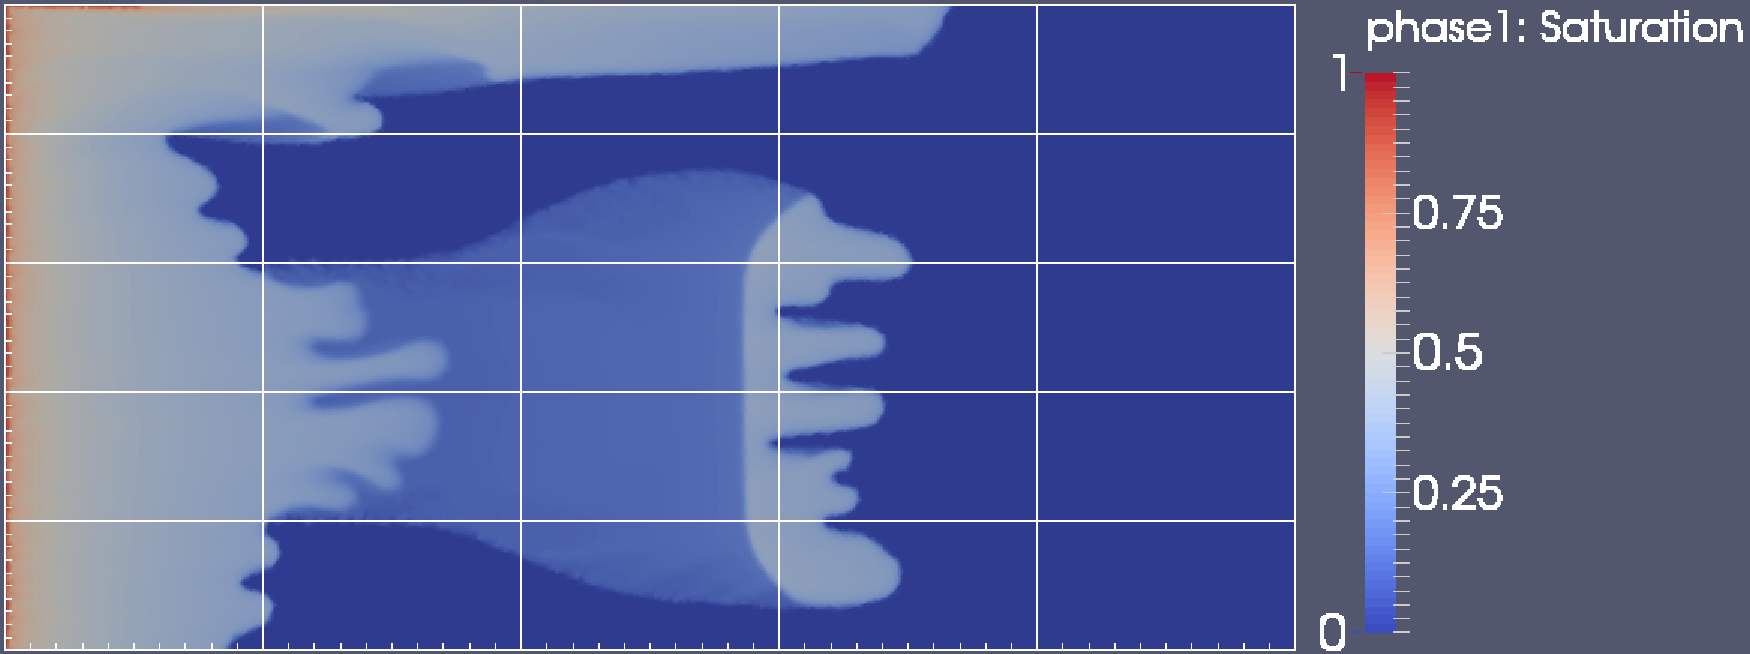
\includegraphics[width=.9\textwidth]{./Pics1/mr10_5regions_adapt/5regions_adapt_500_1.pdf}
}
\vspace{0.0cm}
\hbox{\hspace{6.5cm} (b) flow at t=500 (adaptive mesh)     
}
}     
\caption{At $t=0.25$s ($t=500$, timestemp) cross flow is taking place at the upper part of the formation. The fingers start to becoming more proufound as can been seen at the bottom.}
\label{fig:2testcase_b}
\end{figure}
\end{landscape}
\clearpage



%%%%
%%%%  FIGURE
%%%%
\begin{landscape}
\begin{figure}[ht] 
\vbox{
\hbox{\hspace{3.5cm}
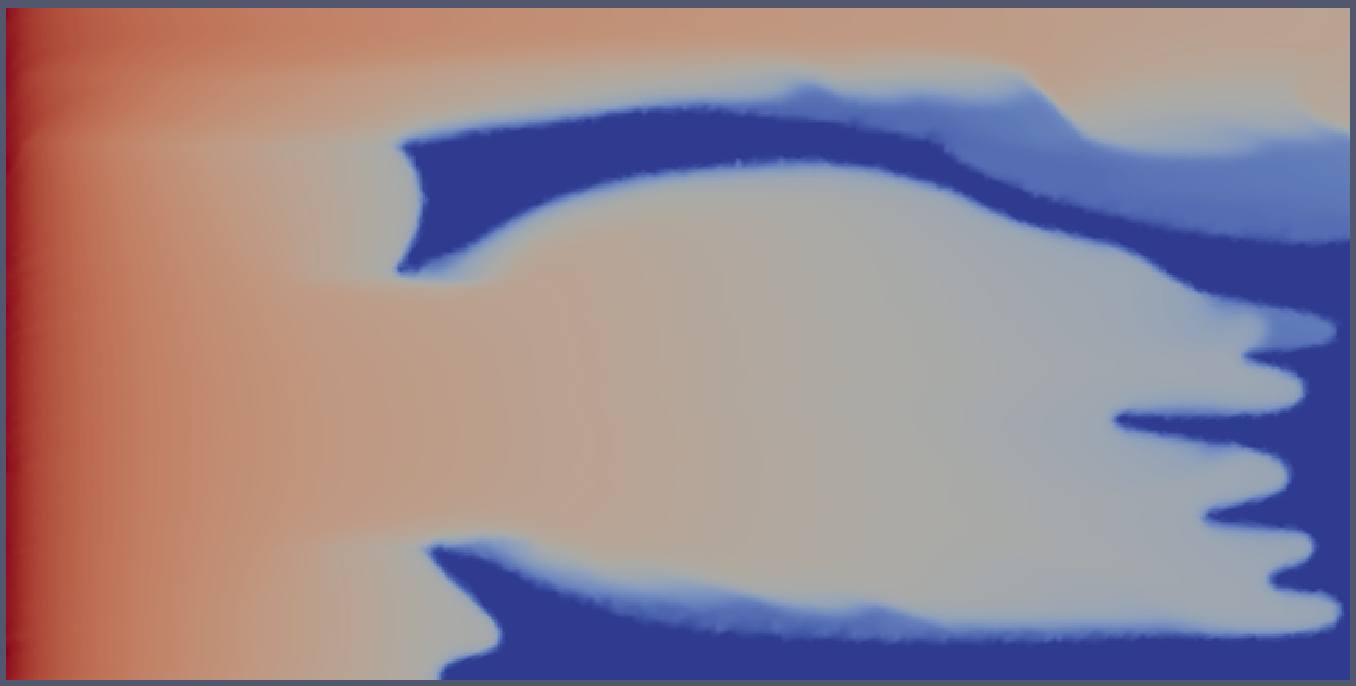
\includegraphics[width=.65\textwidth]{./Pics1/mr10_5regions_fixed/5regions_fixed_1500.pdf} 
}
\vspace{0.0cm}
\hbox{\hspace{6.5cm} (a) flow at t=1500 (fixed mesh)   
}
\vspace{0.25cm}
\hbox{\hspace{3.5cm}
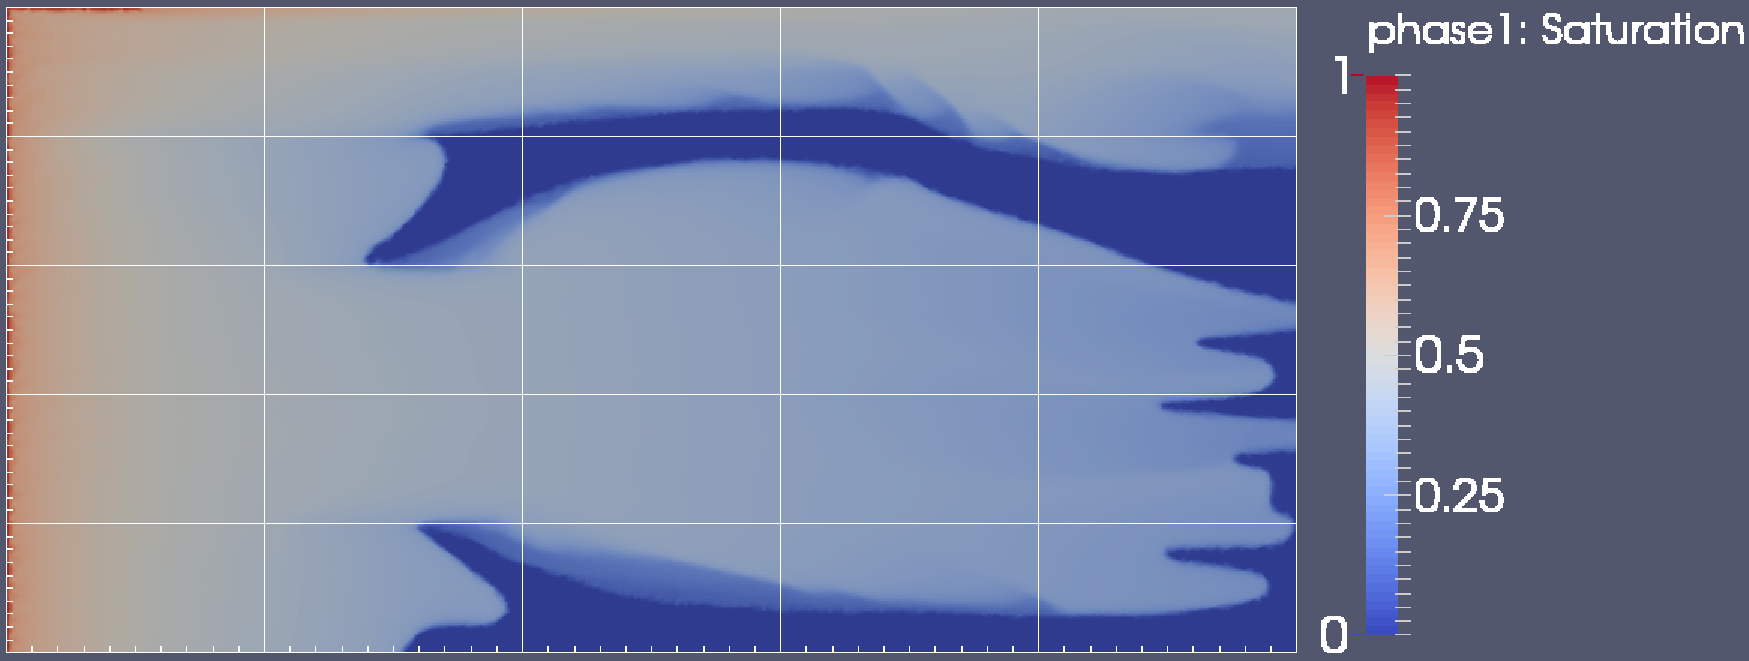
\includegraphics[width=.9\textwidth]{./Pics1/mr10_5regions_adapt/5regions_adapt_1500_1.pdf}
}
\vspace{0.0cm}
\hbox{\hspace{6.5cm} (b) flow at t=1500 (adaptive mesh)     
}
}     
\caption{At $t=0.75 sec$ ($t=1500$, timestemp) the initial cross flow is now fully developed and has travel all the way towards the outlet (right-hand side). and the finger below start forming a front that is also travelling towards the left-hand side.}
\label{fig:2testcase_c}
\end{figure}
\end{landscape}
\clearpage



%%%%
%%%%  FIGURE
%%%%
\begin{landscape}
\begin{figure}[ht] 
\vbox{
\hbox{\hspace{3.5cm}
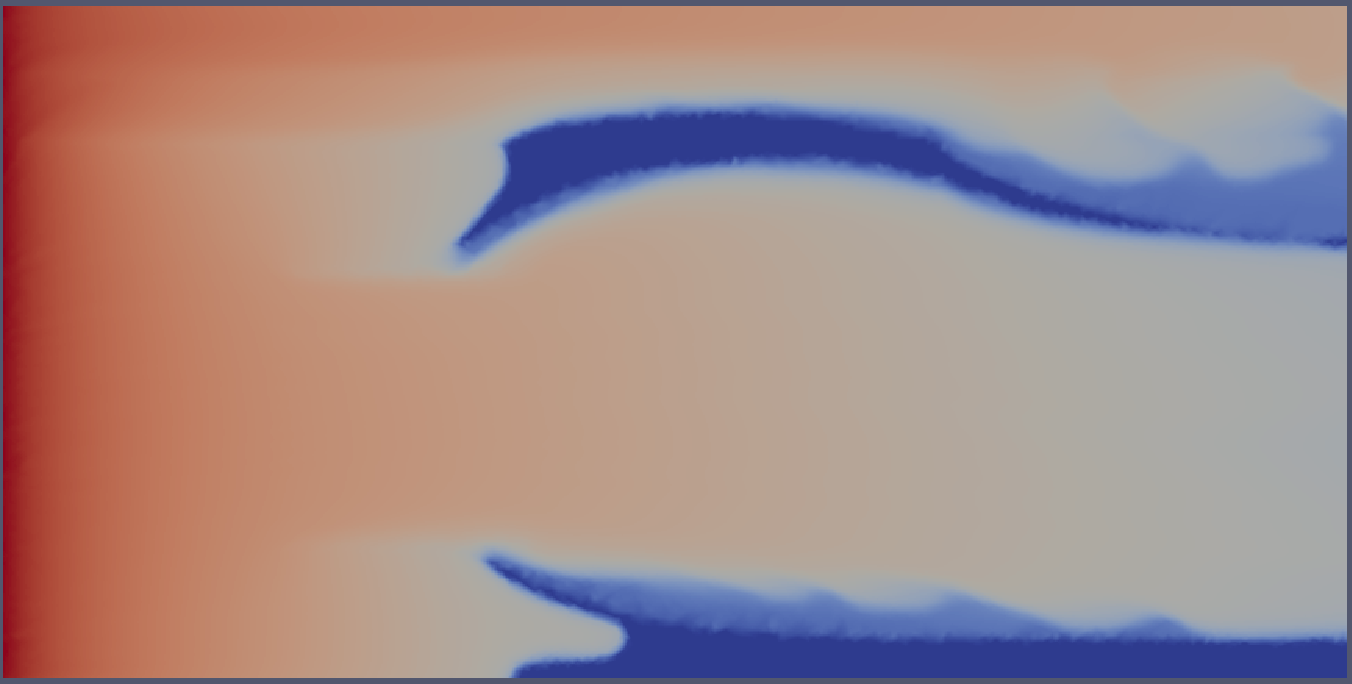
\includegraphics[width=.65\textwidth]{./Pics1/mr10_5regions_fixed/5regions_fixed_2000.pdf} 
}
\vspace{0.0cm}
\hbox{\hspace{6.5cm} (a) flow at t=end (fixed mesh)   
}
\vspace{0.25cm}
\hbox{\hspace{3.5cm}
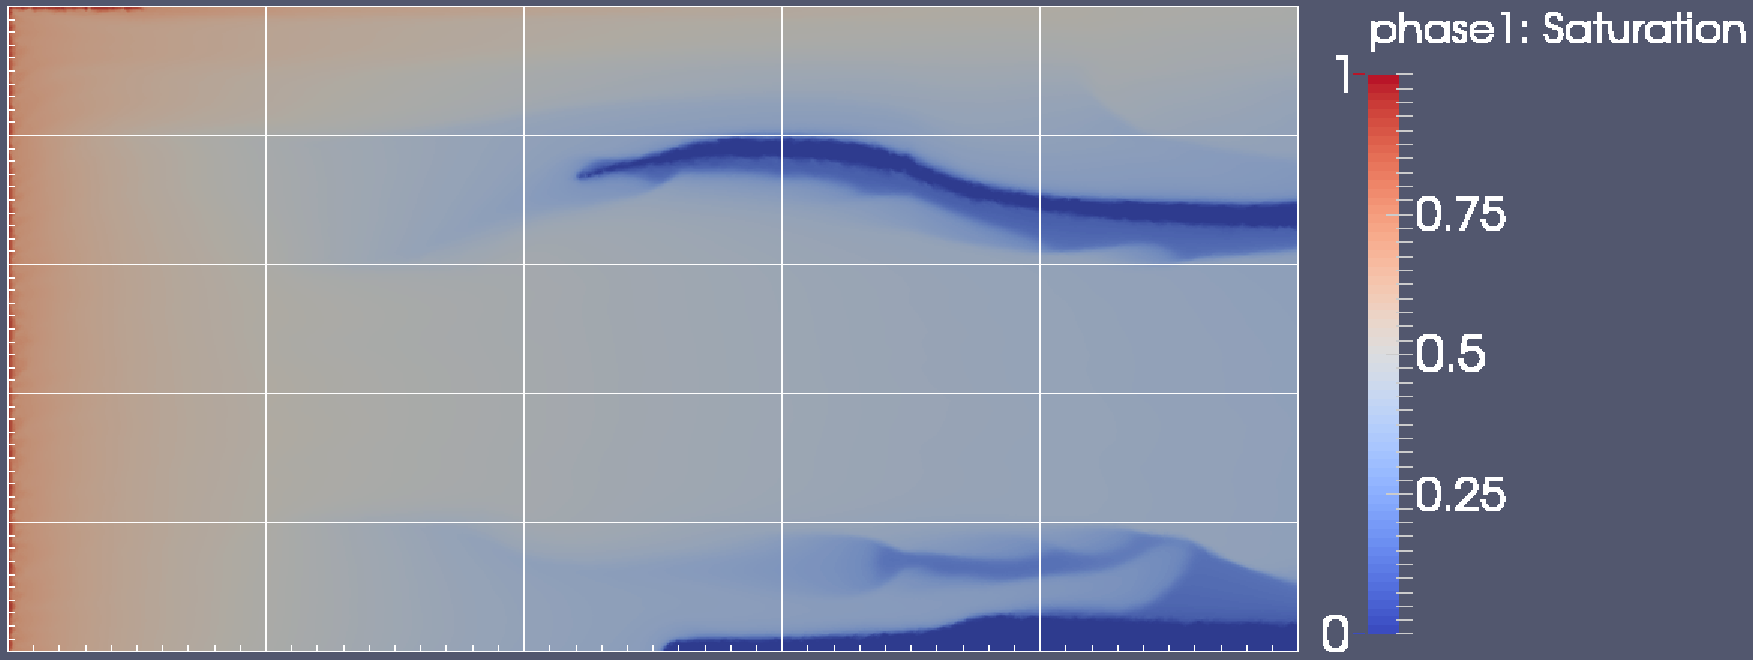
\includegraphics[width=.9\textwidth]{./Pics1/mr10_5regions_adapt/5regions_adapt_3000_1.pdf}
}
\vspace{0.0cm}
\hbox{\hspace{6.5cm} (b) flow at t=end (adaptive mesh)     
}
}     
\caption{Using the $P_{1}DGP_{2}$ element type for VR=$10$ under the same time steps, we compared the impact of fixed and adaptive mesh for the same timeframe. The end of simulation happens at $time=5 sec$ and for the timestemp $t=9999$ while the number of elements in both simulations was approximately $4700$. When adaptive mesh is introduce there is better repersentation of the fluid instabilities as these are developed on time.}
\label{fig:2testcase_d}
\end{figure}
\end{landscape}
\clearpage



%%%%
%%%%  FIGURE
%%%%
\begin{landscape}
\begin{figure}[ht] 
\vbox{
\hbox{\hspace{3.5cm}
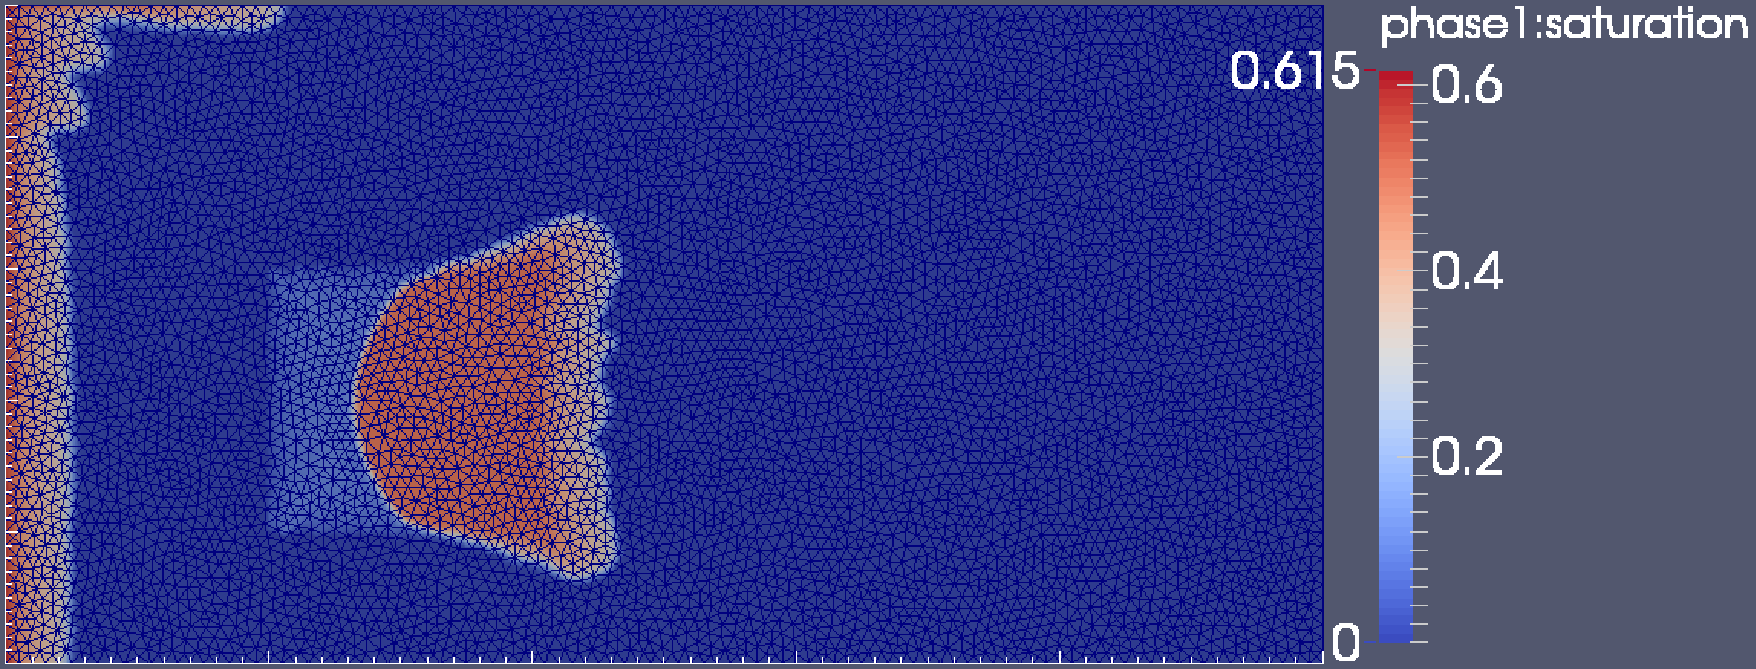
\includegraphics[width=.9\textwidth]{./Pics1/mr10_5regions_fixed_dinlet/5regions_dinlet_fixed_100_1.pdf}
}
\vspace{0.0cm}
\hbox{\hspace{6.5cm} (a) double inlet - fixed mesh   
}
\hbox{\hspace{3.5cm}
  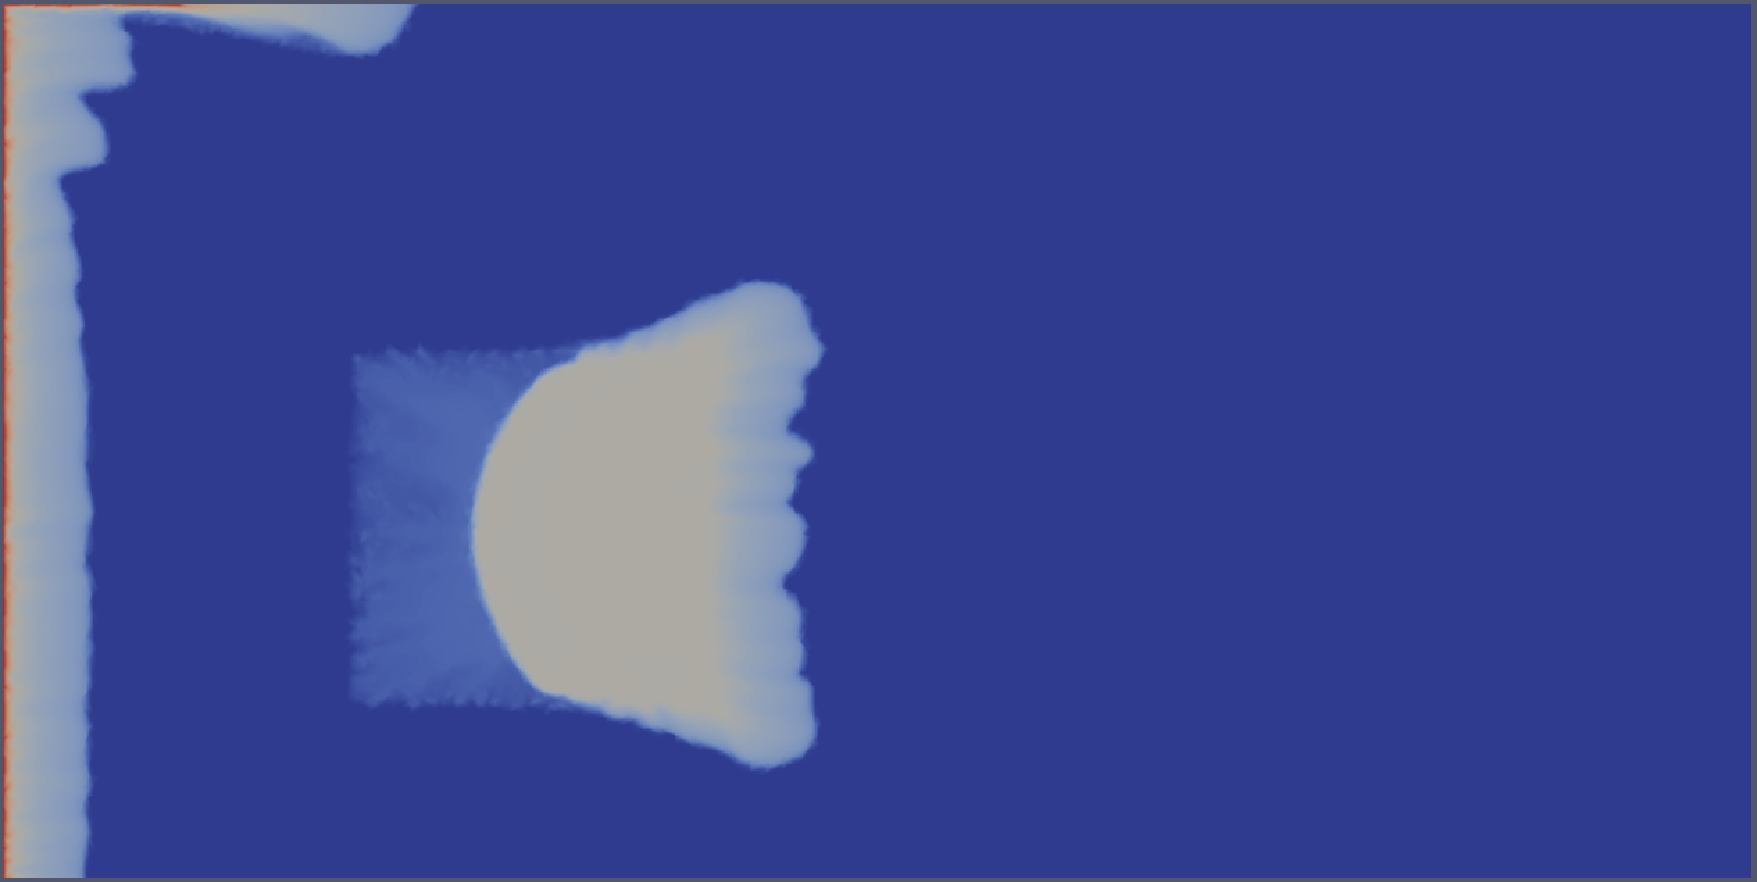
\includegraphics[width=.67\textwidth]{./Pics1/mr10_5regions_adapt_dinlet/5regions_dinlet_adapt_start.pdf}
}
\vspace{0.0cm}
\hbox{\hspace{6.5cm} (b) double inlet adaptive mesh   
}
}     
\caption{Comparing test-cases of fixed and adaptive mesh while a second region/inlet is introduced. For $t=0.101$s, using the $P_{1}DGP_{2}$ element type for MR=$10$ under the same time steps. For this simulation there are $13226$ elements for the fixed messh and $43716$ for the adaptive.}
\label{fig:3testcase_a}
\end{figure}
\end{landscape}
\clearpage

%%%%
%%%%  FIGURE
%%%%
\begin{figure}[ht] 
\vbox{
\hbox{\hspace{3.5cm}
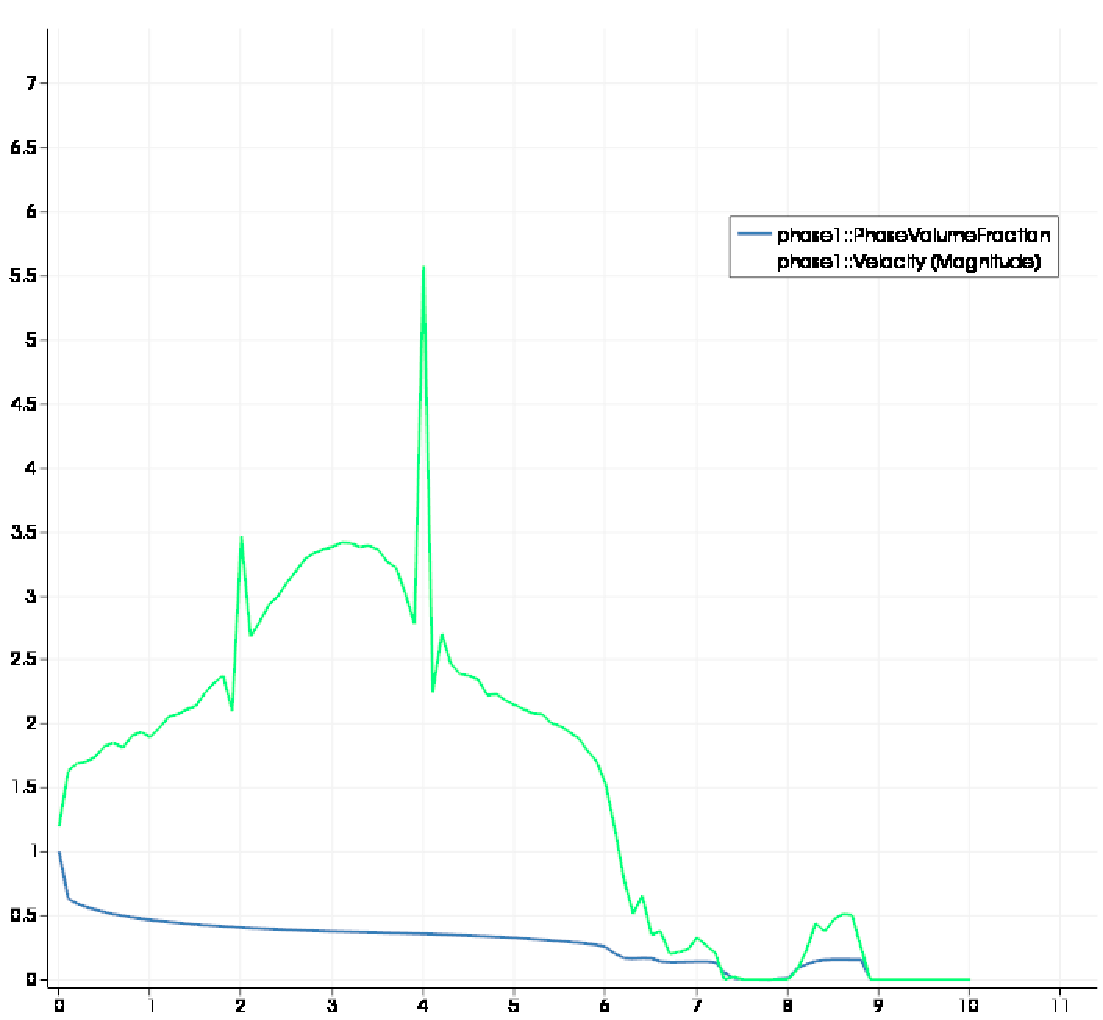
\includegraphics[width=.5\textwidth]{./Pics1/mr10_5regions_adapt/5regions_adapt_vel_magn.pdf} 
}
\vspace{0.0cm}
\hbox{\hspace{5.0cm} (a) single inlet velocity magnitude   
}
\hbox{\hspace{3.5cm}
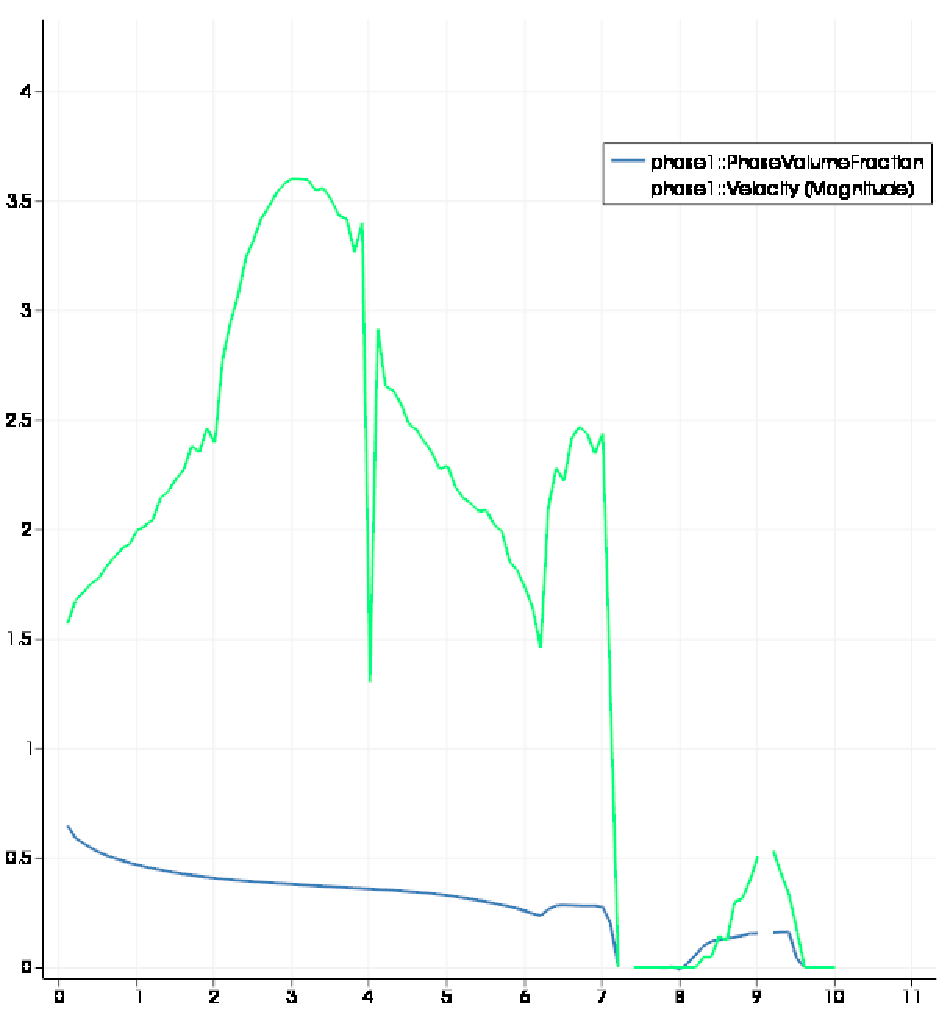
\includegraphics[width=.5\textwidth]{./Pics1/mr10_5regions_adapt_dinlet/5regions_dinlet_adapt_vel_magn.pdf}
}
\vspace{0.0cm}
\hbox{\hspace{5.0cm} (b) double inlet velocity magnitude   
}
}     
\caption{For the same time step, t=1000, these plots describe the velocity magnitudes of the phase $1$ (injected fluid) under the same boundary and initiall conditions. From top to bottom,these graphs describe the velocity magnitude %for fixed mesh is plotted(top), the velocity magnitude 
for adaptive mesh-single inlet (top) and the velocity magnitude for adaptive mesh with double inlet (bottom) as these are also presented in fig.\ref{fig:3testcase_a}. The main difference between the upper and lower plot %is not just the ability to capture in greater detail, the fluid instabilities as they happenduring the finger development and their velocity patterns. While there 
is the impact of the second injection interval as this can be seen from the slope and the rate that the velocity magnitude is changing.}
\label{fig:vel_magn}
\end{figure}

%%%%
%%%%  FIGURE
%%%%
\begin{landscape}
\begin{figure}[ht] 
\vbox{
\hbox{\hspace{3.5cm}
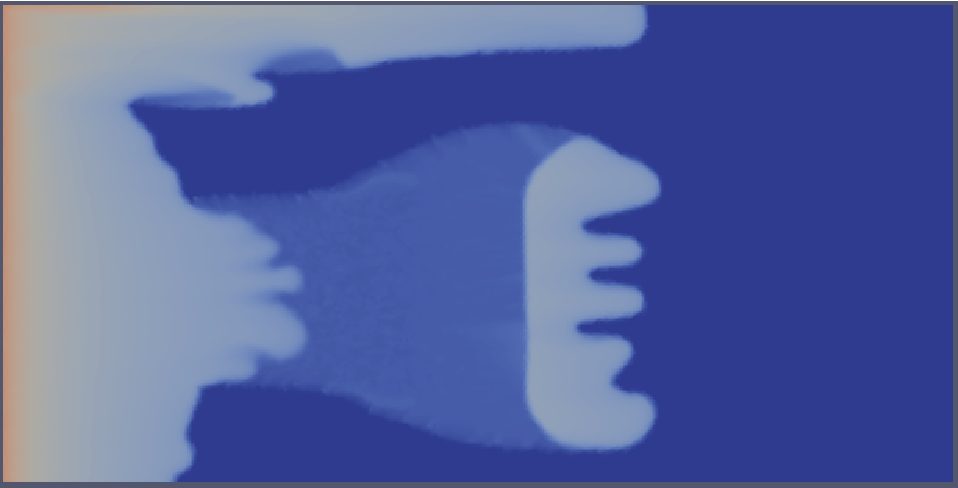
\includegraphics[width=.65\textwidth]{./Pics1/5reg_dinlet_fixed_500.pdf} 
}
\vspace{0.0cm}
\hbox{\hspace{6.5cm} (a) double inlet - fixed mesh   
}
\hbox{\hspace{3.5cm}
\includegraphics[width=.9\textwidth]{./Pics1/5reg_dinlet_adapt_500_1.pdf}
}
\vspace{0.0cm}
\hbox{\hspace{6.5cm} (b) double inlet adaptive mesh   
}
}     
\caption{For $t=5$s there is a comparison between fixed mesh(a) and adaptive mesh(b).}
\label{fig:3testcase_b}
\end{figure}
\end{landscape}
\clearpage

%%%%
%%%%  FIGURE
%%%%
\begin{landscape}
\begin{figure}[ht] 
\vbox{
\hbox{\hspace{3.5cm}
\includegraphics[width=.65\textwidth]{./Pics1/5reg_dinlet_fixed_1500.pdf} 
}
\vspace{0.0cm}
\hbox{\hspace{6.5cm} (a) double inlet - fixed mesh   
}
\hbox{\hspace{3.5cm}
\includegraphics[width=.9\textwidth]{./Pics1/5reg_dinlet_adapt_1500_1.pdf}
}
\vspace{0.0cm}
\hbox{\hspace{6.5cm} (b) double inlet adaptive mesh   
}
}     
\caption{For $t=7.5$s this is a comparison between fixed mesh(a) and adaptive mesh(b).}
\label{fig:3testcase_c}
\end{figure}
\end{landscape}
\clearpage

%%%%
%%%%  FIGURE
%%%%
\begin{landscape}
\begin{figure}[ht] 
\vbox{
\hbox{\hspace{3.5cm}
\includegraphics[width=.65\textwidth]{./Pics1/5reg_dinlet_fixed_end.pdf} 
}
\vspace{0.0cm}
\hbox{\hspace{6.5cm} (a) double inlet - fixed mesh   
}
\hbox{\hspace{3.5cm}
\includegraphics[width=.9\textwidth]{./Pics1/5reg_dinlet_adapt_end_1.pdf}
}
\vspace{0.0cm}
\hbox{\hspace{6.5cm} (b) double inlet adaptive mesh   
}
}     
\caption{This is a comparison between fixed mesh(a) and adaptive mesh(b) at the end of the simulation. For the fixed mesh at this point the maximum number of point is $13226$ while for the adaptive mesh is $7582$ and most of them are located where is needed in the domain.}
\label{fig:3testcase_d}
\end{figure}
\end{landscape}
\clearpage

%%%%
%%%%  FIGURE
%%%%
\begin{landscape}
\begin{figure}[ht] 
\vbox{
\hbox{\hspace{3.5cm}
\includegraphics[width=.8\textwidth]{./Pics1/mr100_fixed/mr100_fixed_500.pdf} 
}
\vspace{0.0cm}
\hbox{\hspace{4.0cm} (a) fixed and unstructured mesh for MR = 100 (start)   
}
\hbox{\hspace{3.5cm}
\includegraphics[width=.8\textwidth]{./Pics1/mr100_fixed/mr100_fixed_1500.pdf}
}
\vspace{0.0cm}
\hbox{\hspace{3.75cm} (b) fixed and unstructured mesh for MR = 100 (t = 1500)   
}
}     
\caption{For the case of VR=$100$ from top to bottom, the number of elements is $4680$ and fixed and unstructured mesh for the same time steps, t=$0.25$ or t=500(a), t=$0.75$ or t=1500(b). }
\label{fig:4testcase_a}
\end{figure}
\end{landscape}
\clearpage

%%%%
%%%%  FIGURE
%%%%
\begin{landscape}
\begin{figure}[ht] 
\vbox{
\hbox{\hspace{3.5cm}
\includegraphics[width=.8\textwidth]{./Pics1/mr100_fixed/mr100_fixed_3000.pdf} 
}
\vspace{0.0cm}
\hbox{\hspace{3.75cm} (c) fixed and unstructured mesh for MR = 100    
}
\hbox{\hspace{3.5cm}
\includegraphics[width=.8\textwidth]{./Pics1/mr100_fixed/mr100_fixed_end.pdf}
}
\vspace{0.0cm}
\hbox{\hspace{7.cm} (d) end of simulations     
}
}     
\caption{screenshot (c) is for t=$1.5$ sec or t=$3000$ and screenshot (d) is for t=$3.175$ sec, at the end of the simulations. }
\label{fig:4testcase_b}
\end{figure}
\end{landscape}
\clearpage


 

\end{document}
%% End of tex file.


